% !TeX root = ../tesis.tex
%%%%%%%%%%%%%%%%%%%%%%%%%%%%%%%%%%%%%%%%%%%%%%%%%%%%%%%%%%%%%%%%%%%
% ANEXO F — Recursos Visuales Analíticos: Red Actual de la ZMVM
%
% Dos fuentes de visualización:
%   F.1  Cartografía QGIS     → Figures/Mapas/Qgis_Resources/RedActual/
%   F.2  Tableros Apimetro    → Figures/Mapas/Tableau_Resources/RedActual/Apimetro/
%   F.3  Tableros Modelo VFT  → Figures/Mapas/Tableau_Resources/RedActual/VFTModel/
%%%%%%%%%%%%%%%%%%%%%%%%%%%%%%%%%%%%%%%%%%%%%%%%%%%%%%%%%%%%%%%%%%%

Este anexo reúne los recursos visuales analíticos generados durante el procesamiento
de la red de transporte actual de la \zmvm{}. A diferencia del Anexo~E, que contiene
los mapas de presentación para el jurado, este anexo sirve como referencia técnica
completa para los capítulos de análisis. Cada figura está vinculada a uno o más
indicadores del Capítulo~\ref{ch:analisis-red-actual}.

Los mapas cartográficos provienen de \textbf{QGIS~3.x} con proyección
\textsc{epsg}:32614 (UTM zona~14N). Los tableros y gráficas fueron producidos
con \textbf{Tableau Desktop 2026.1} a partir de los \textit{GeoPackages} exportados
por el Modelo VFT y los \textit{feeds} \gtfs{} de \textbf{Apimetro}.

% =============================================================================
\section{Cartografía \textsc{QGIS} — Red Actual}
\label{anx:f-qgis-red-actual}
% =============================================================================

% --- F.1.1 -------------------------------------------------------------------
\subsection{Red de Transporte Público de la \zmvm}
\label{anx:f-qgis-transporte}

\begin{figure}[p]
  \centering
  \includegraphics[width=\textwidth]{Figures/Mapas/Qgis_Resources/RedActual/Mapa_Transporte_Publico}
  \caption[Red de transporte público de la \zmvm{} — capa base]{Capa base de
  la red de transporte público de la \zmvm{}, con los doce sistemas representados
  por color de modo. Sirve como referencia geográfica de los indicadores del
  Capítulo~\ref{ch:analisis-red-actual}.}
  \label{fig:anx-f-qgis-transporte}
  \fuentefigura{Elaboración propia con \textbf{Transport-gis-zmvm-mjg};
    datos: \gtfs{} \textsc{semovi} 2024 e \textsc{inegi} 2023.}
\end{figure}

% --- F.1.2 -------------------------------------------------------------------
\subsection{Red Esquemática del Grafo Topológico}
\label{anx:f-qgis-red-esquematica}

\begin{figure}[p]
  \centering
  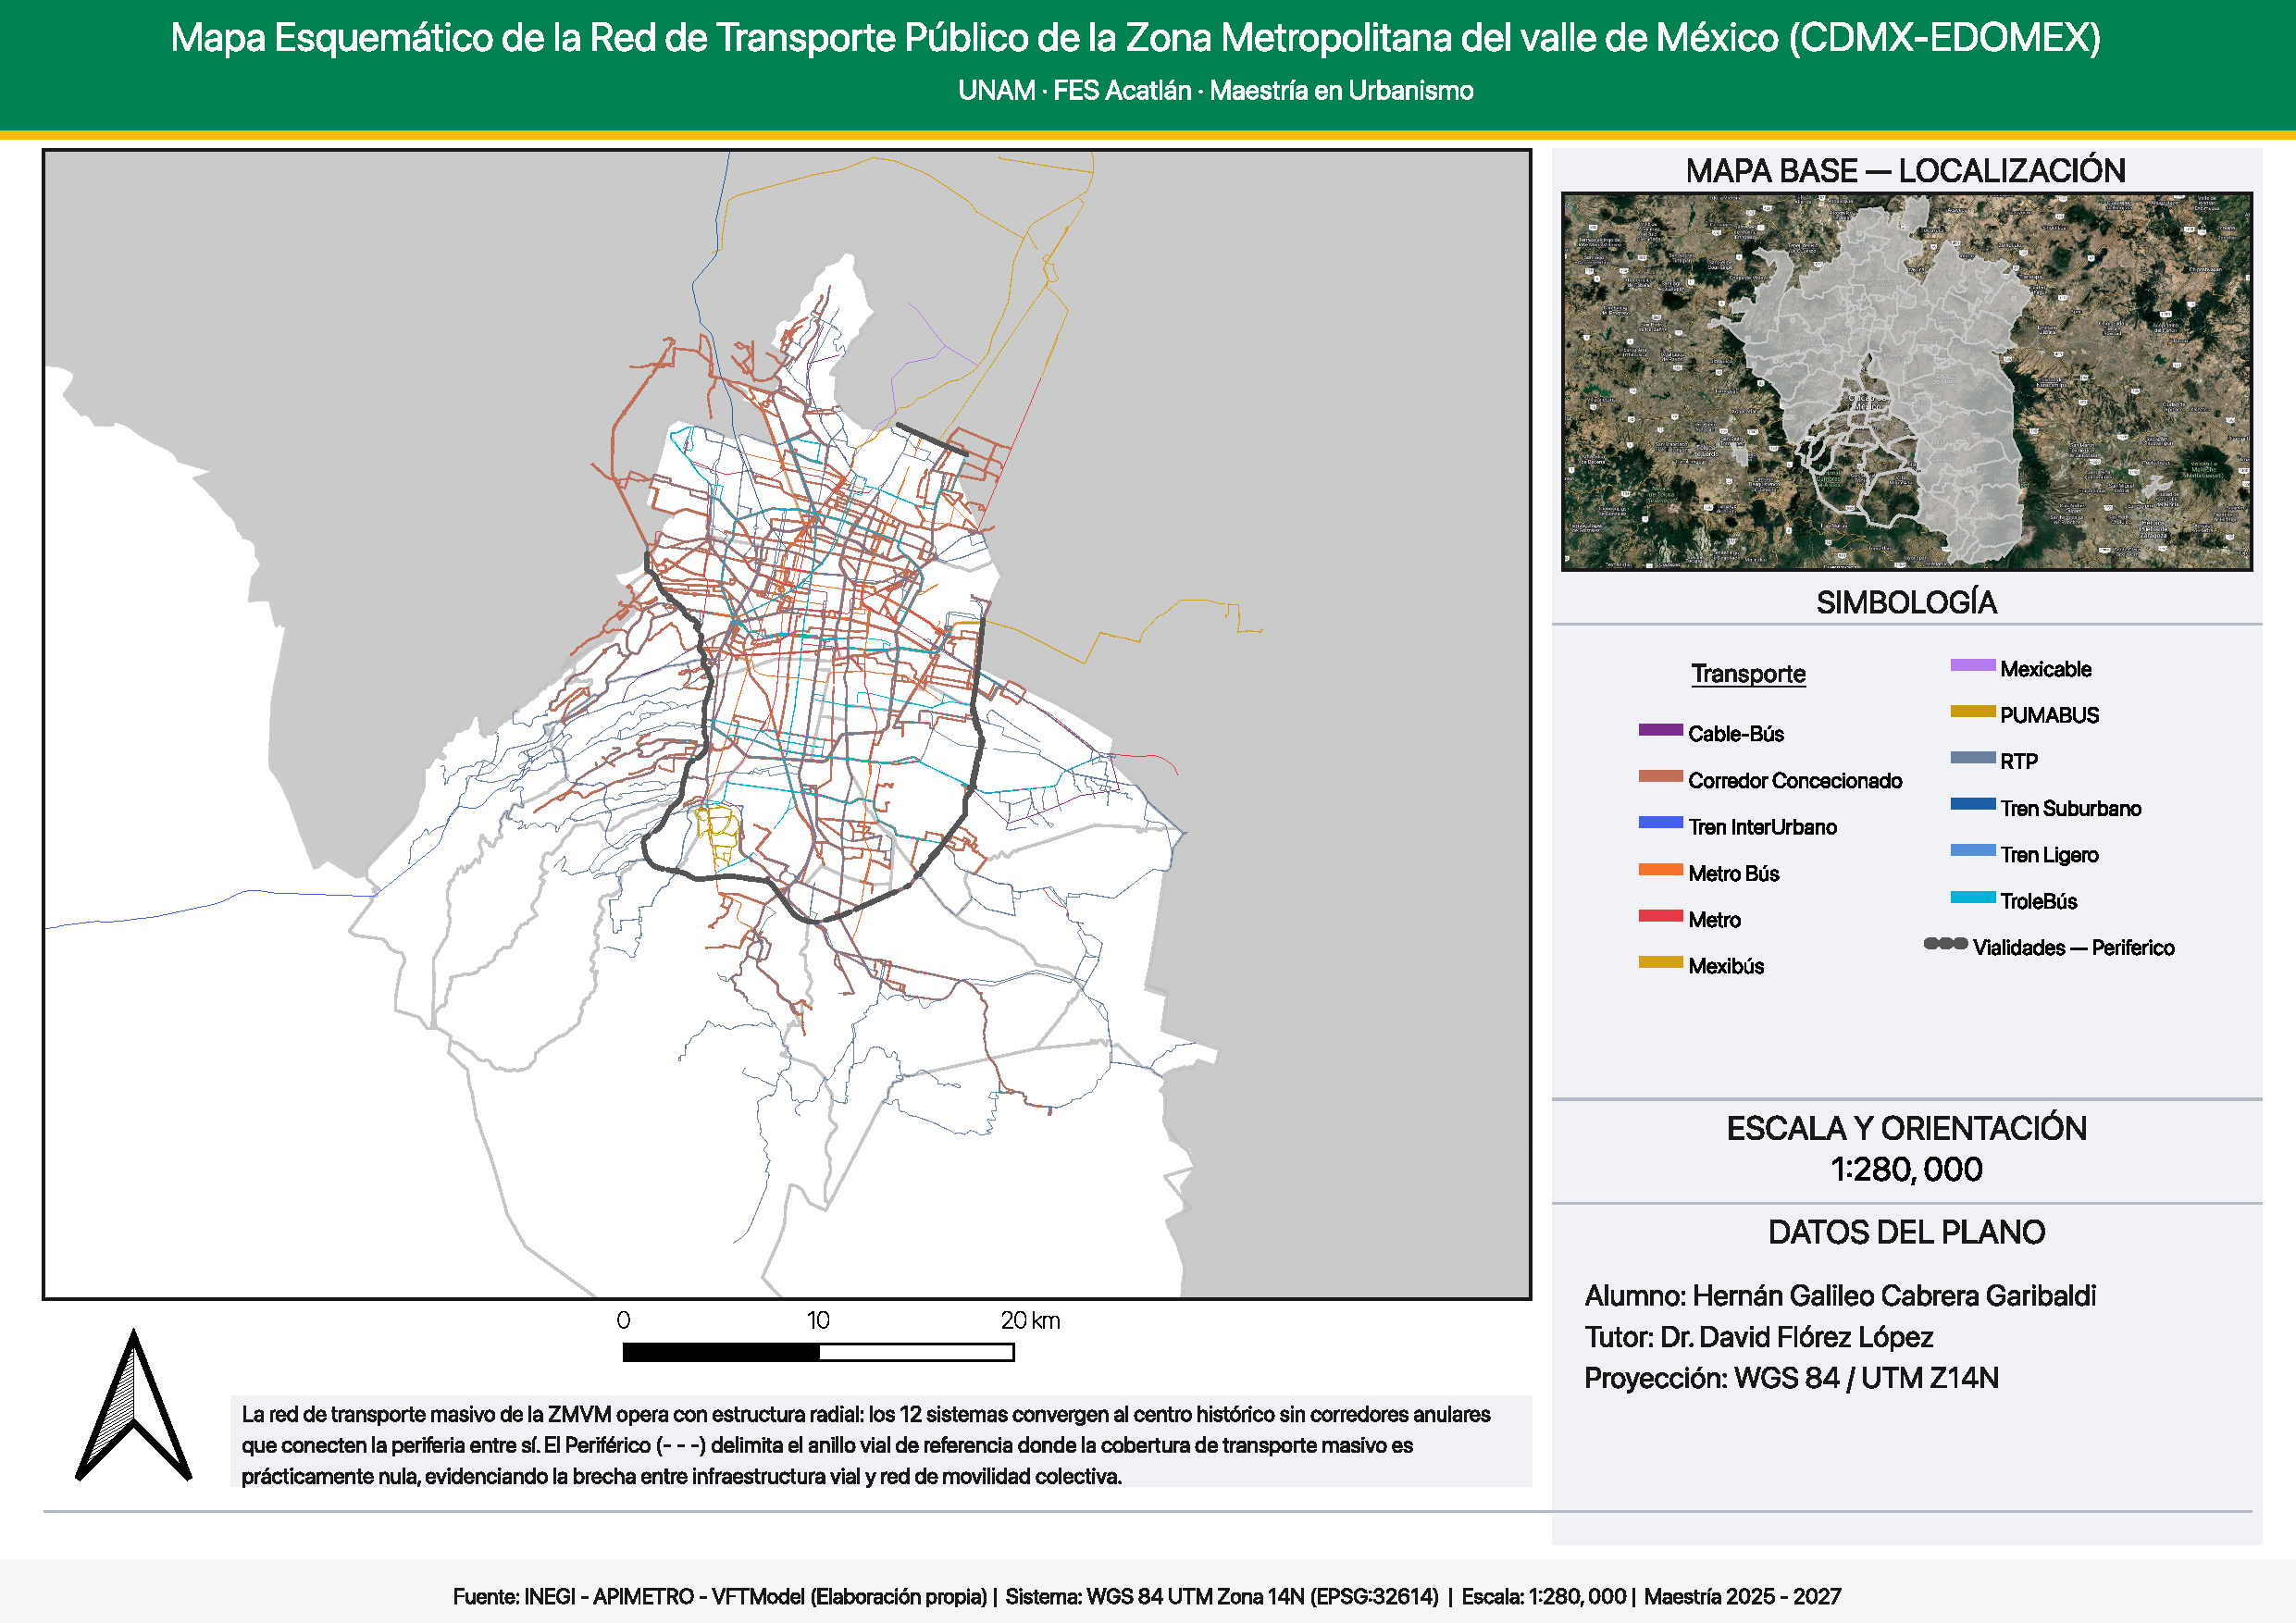
\includegraphics[width=\textwidth]{Figures/Mapas/Qgis_Resources/RedActual/Mapa_Red_Esquematica}
  \caption[Grafo topológico multimodal de la \zmvm{} — red esquemática]{Representación
  esquemática del grafo dirigido construido por el Modelo VFT sobre la red multimodal
  de la \zmvm{}. Cada nodo corresponde a una estación topológica tras el proceso de
  \termino{snapping} con árbol \texttt{KDTree} (tolerancia 85~m);
  cada arista representa un segmento de servicio real o un enlace de transbordo
  peatonal generado algorítmicamente.}
  \label{fig:anx-f-qgis-red}
  \fuentefigura{Elaboración propia con \textbf{Transport-gis-zmvm-mjg};
    datos: \gtfs{} \textsc{semovi} 2024 e \textsc{inegi} 2023.}
\end{figure}

% --- F.1.3 -------------------------------------------------------------------
\subsection{Cobertura Espacial — Isócronas de 800~m}
\label{anx:f-qgis-cobertura-total}

\begin{figure}[p]
  \centering
  
\includegraphics[width=\textwidth]{Figures/Mapas/Qgis_Resources/RedActual/Mapa_Cobertura_Red_Total}
  \caption[Cobertura espacial de la red — isócronas 800~m, alta resolución]{Cobertura
  espacial del indicador $C$ calculado por el Modelo VFT. El área sombreada representa
  la zona alcanzable a 800~m de caminata desde cualquier parada o estación
  (isócrona peatonal equivalente a 10--15~min). Las zonas sin cobertura
  revelan los municipios y alcaldías con mayor déficit de acceso estructurado al
  transporte público.}
  \label{fig:anx-f-qgis-cobertura-total}
  \fuentefigura{Elaboración propia con \textbf{Transport-gis-zmvm-mjg};
    datos: \gtfs{} \textsc{semovi} 2024 e \textsc{inegi} 2023.}
\end{figure}

% --- F.1.4 -------------------------------------------------------------------
\subsection{Cobertura Espacial — Mapa de Calor}
\label{anx:f-qgis-cobertura-calor}

\begin{figure}[p]
  \centering
  
\includegraphics[width=\textwidth]{Figures/Mapas/Qgis_Resources/RedActual/Mapa_Cobertura_Mapa_Calor}
  \caption[Densidad de cobertura de la red — mapa de calor, alta resolución]{Densidad
  de la cobertura espacial representada como mapa de calor. La intensidad refleja
  la superposición de isócronas de distintos sistemas: los núcleos de mayor
  temperatura corresponden a zonas con acceso simultáneo a tres o más modos de
  transporte, mientras que las áreas frías indican escasa o nula cobertura multimodal.}
  \label{fig:anx-f-qgis-cobertura-calor}
  \fuentefigura{Elaboración propia con \textbf{Transport-gis-zmvm-mjg};
    datos: \gtfs{} \textsc{semovi} 2024 e \textsc{inegi} 2023.}
\end{figure}

% --- F.1.5 -------------------------------------------------------------------
\subsection{Fuerza Capilar — Macrohubs Principales}
\label{anx:f-qgis-fuerza-capilar}

\begin{figure}[p]
  \centering
  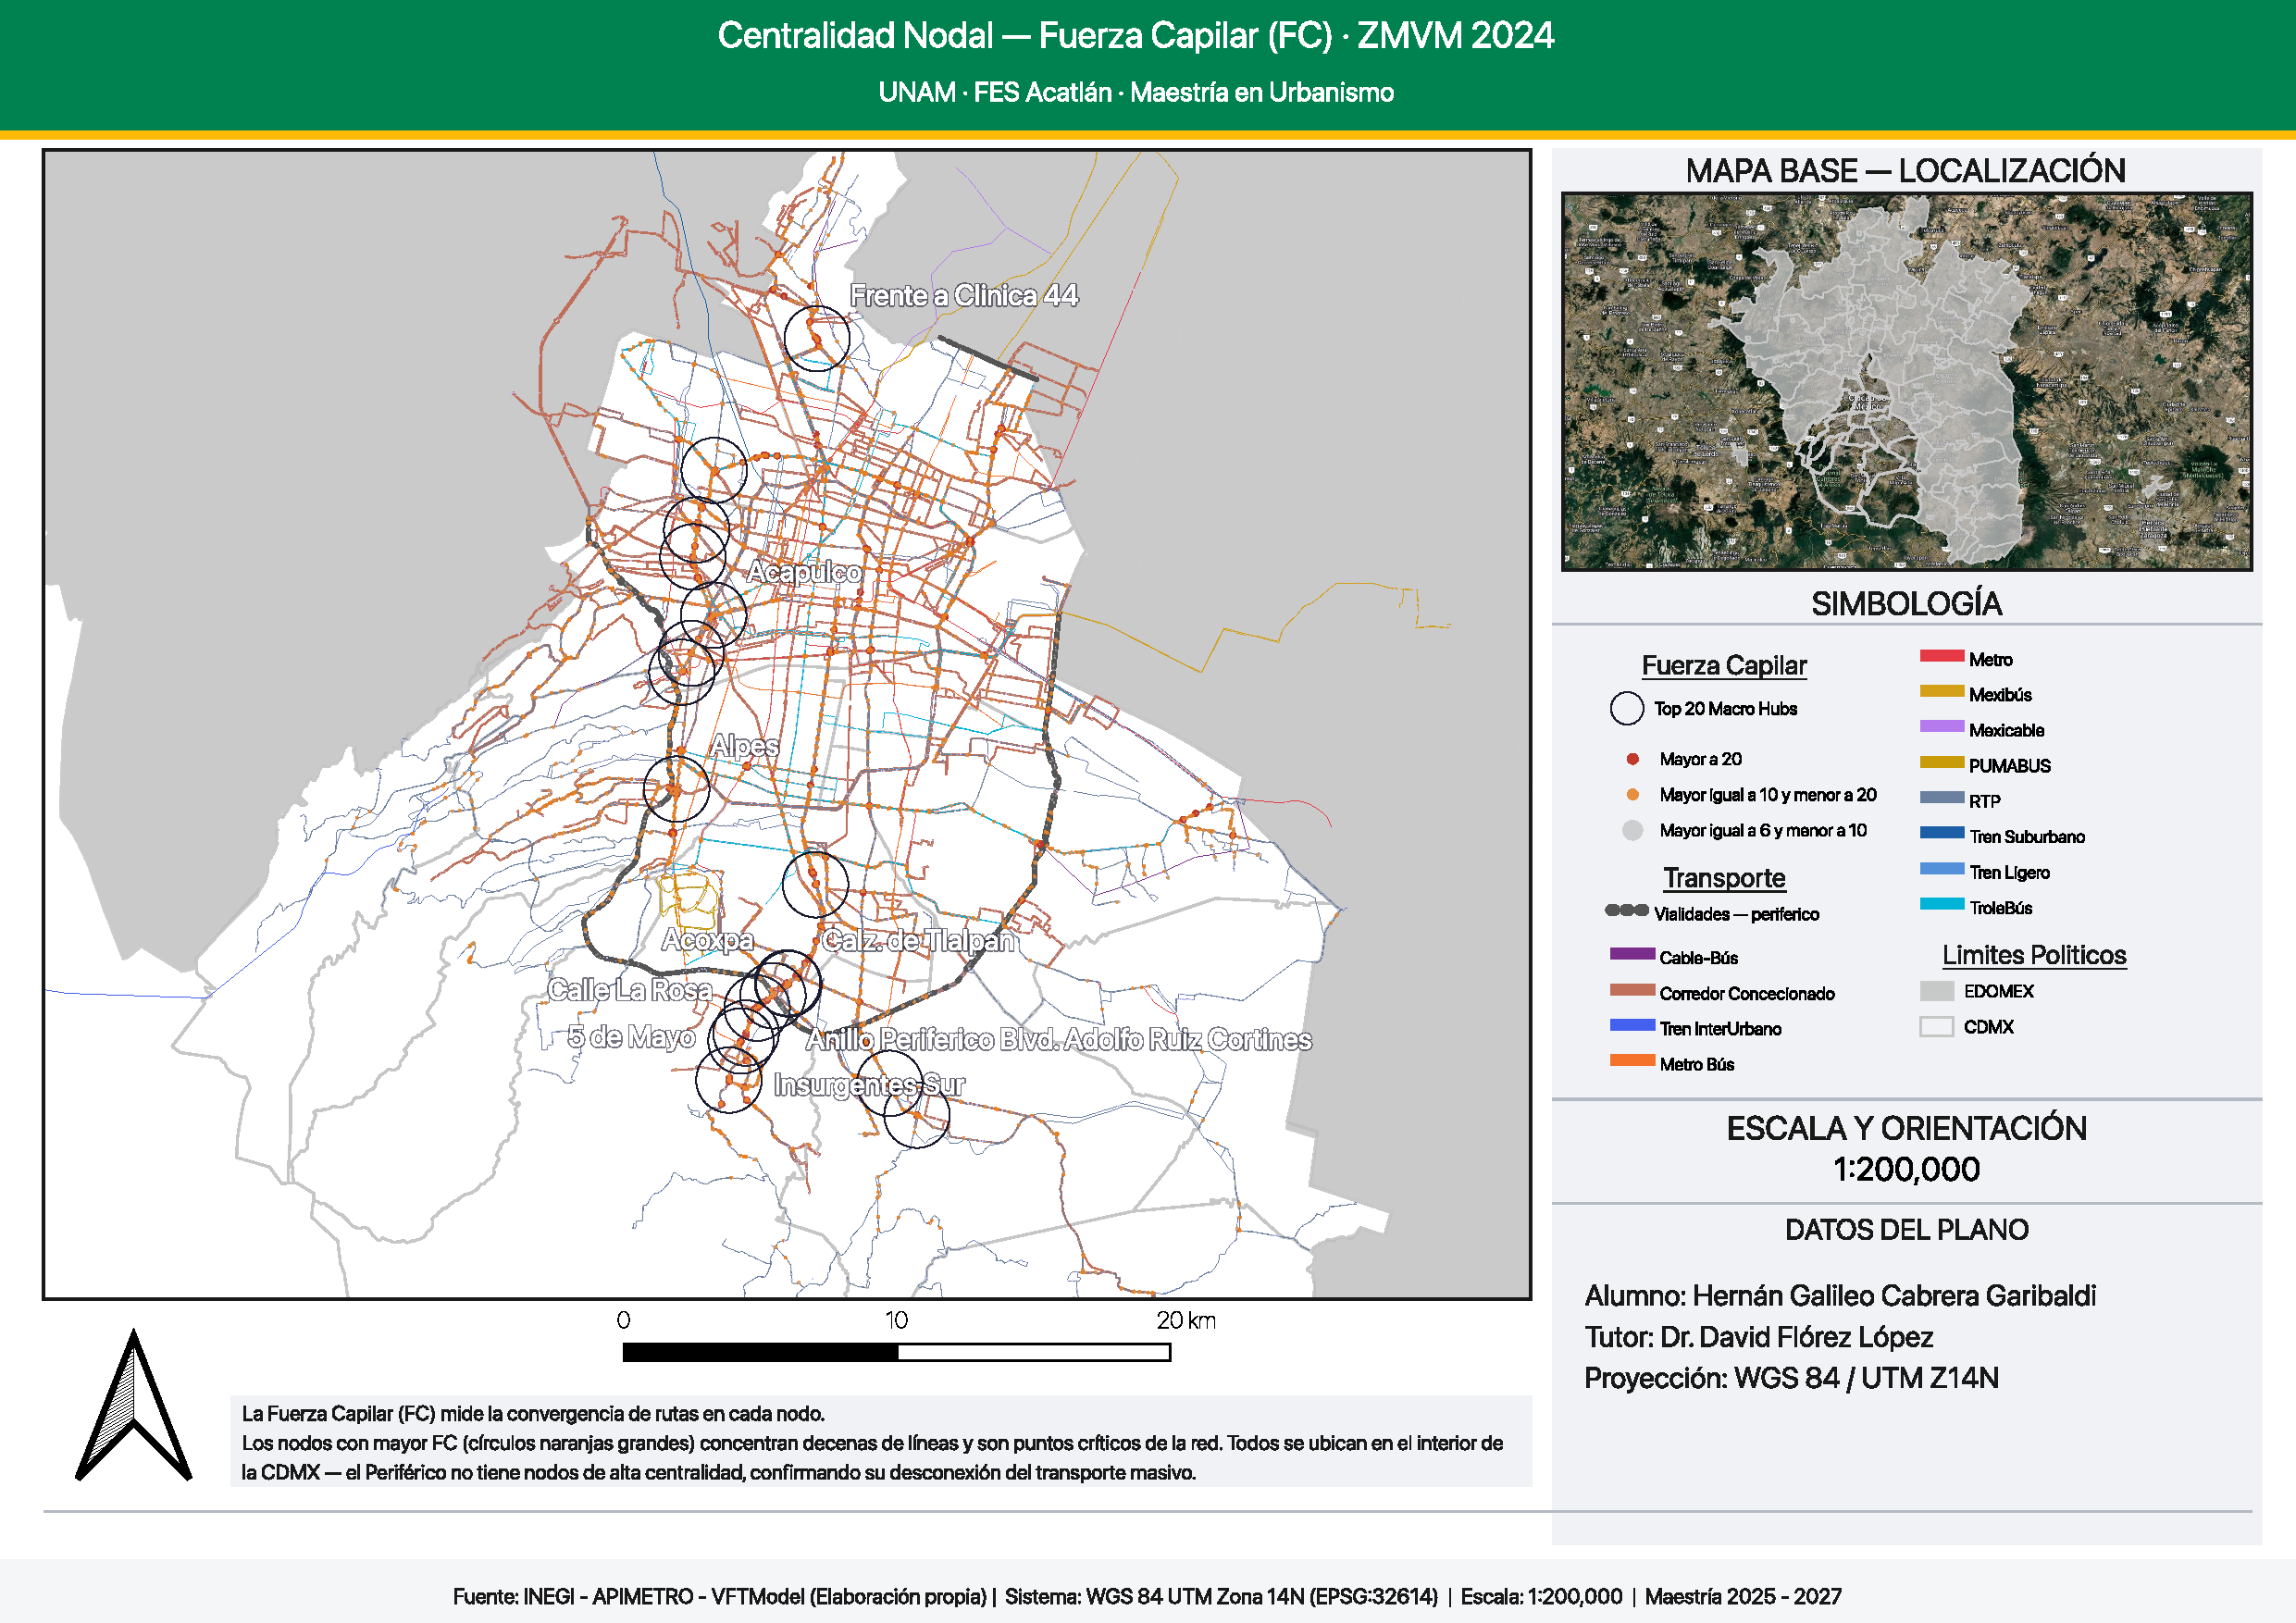
\includegraphics[width=\textwidth]{Figures/Mapas/Qgis_Resources/RedActual/Mapa_Fuerza_Capilar}
  \caption[Fuerza capilar $FC_h$ — concentración de macrohubs, alta resolución]{Distribución
  espacial del indicador de Fuerza Capilar $FC_h$ sobre la red de la \zmvm{}.
  El tamaño y color de cada punto reflejan el valor de $FC_h$: los nodos con mayor
  puntuación agrupan el mayor número de paradas de distintos sistemas en un radio
  de 100~m, constituyendo los puntos de mayor redistribución de flujos en la red
  multimodal.}
  \label{fig:anx-f-qgis-fuerza-capilar}
  \fuentefigura{Elaboración propia con \textbf{Transport-gis-zmvm-mjg};
    datos: \gtfs{} \textsc{semovi} 2024 e \textsc{inegi} 2023.}
\end{figure}

% --- F.1.6 -------------------------------------------------------------------
\subsection{Factor de Desviación por Nodo}
\label{anx:f-qgis-df}

\begin{figure}[p]
  \centering
  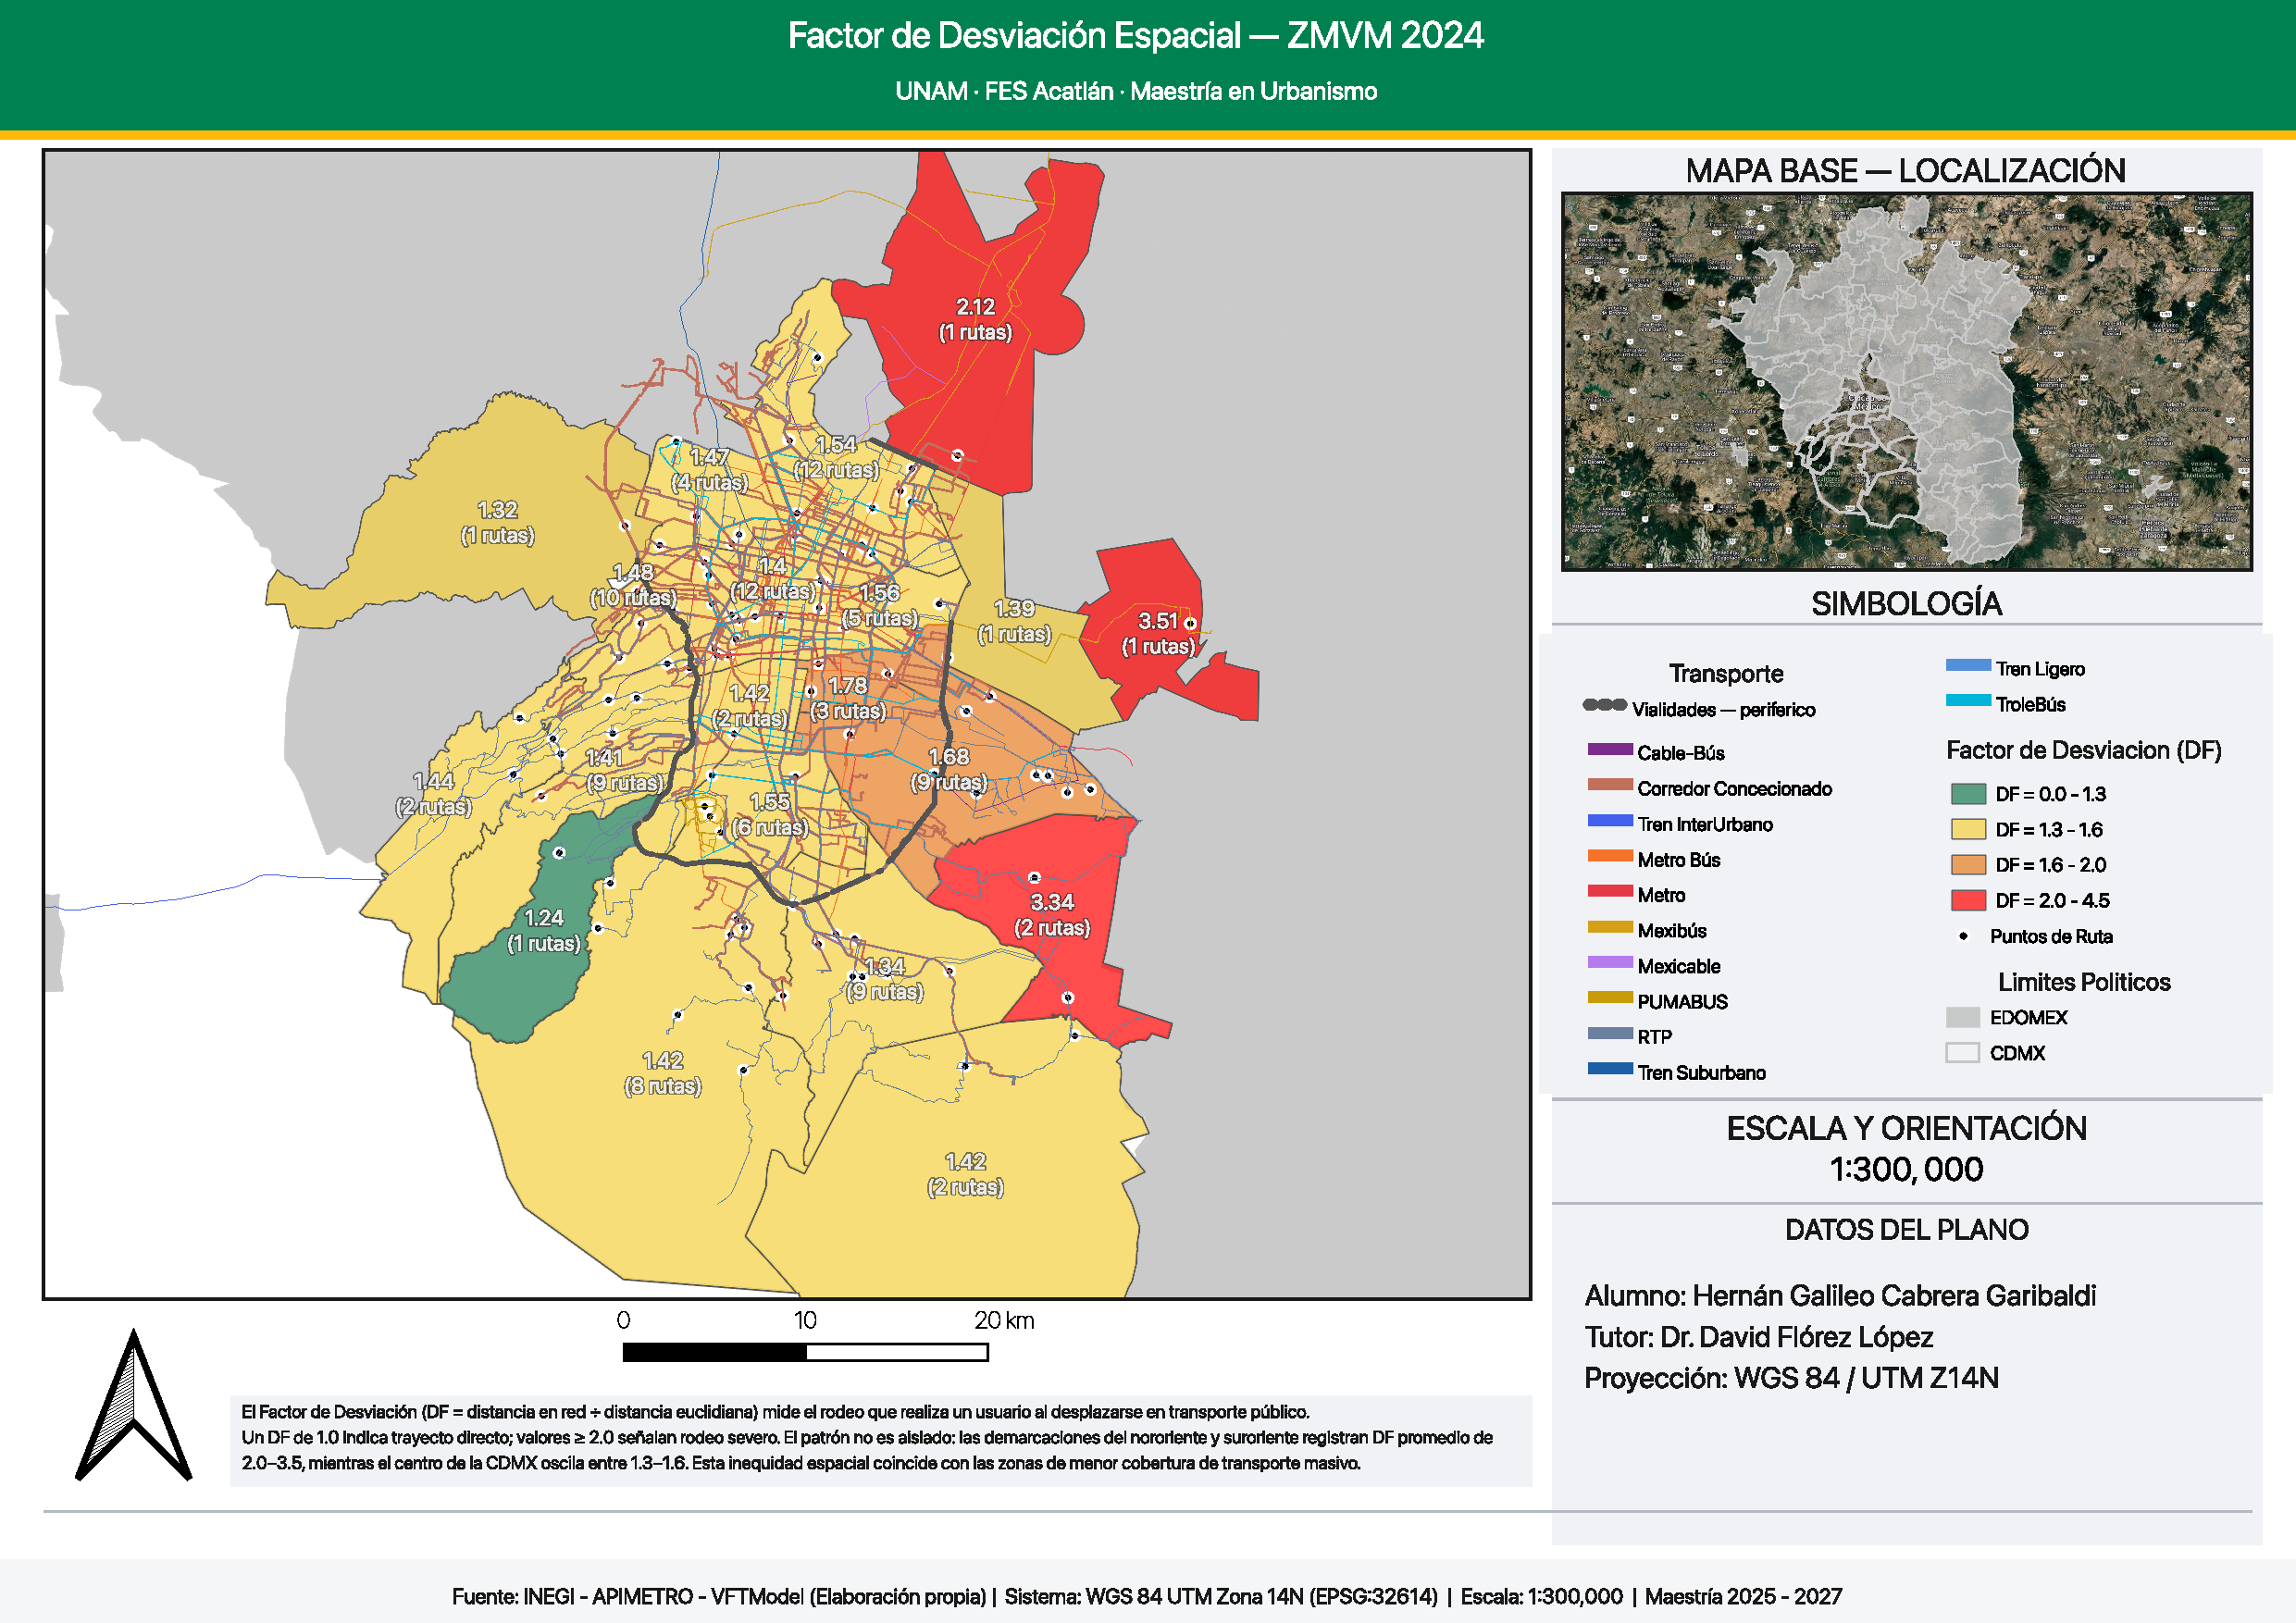
\includegraphics[width=\textwidth]{Figures/Mapas/Qgis_Resources/RedActual/Mapa_DF}
  \caption[Factor de desviación $DI$ por nodo — alta resolución]{Factor de
  desviación ($DI$) calculado sobre una muestra de 100 rutas aleatorias.
  El gradiente de color (verde → rojo) indica la relación entre la distancia
  real de viaje y la distancia euclidiana óptima: los nodos rojos corresponden
  a zonas donde las rutas disponibles obligan a desvíos significativos respecto
  al trayecto más directo posible.}
  \label{fig:anx-f-qgis-df}
  \fuentefigura{Elaboración propia con \textbf{Transport-gis-zmvm-mjg};
    datos: \gtfs{} \textsc{semovi} 2024 e \textsc{inegi} 2023.}
\end{figure}

% --- F.1.7 -------------------------------------------------------------------
\subsection{Centralidad de Intermediación \texorpdfstring{$B(v)$}{B(v)}}
\label{anx:f-qgis-betweenness}

\begin{figure}[p]
  \centering
  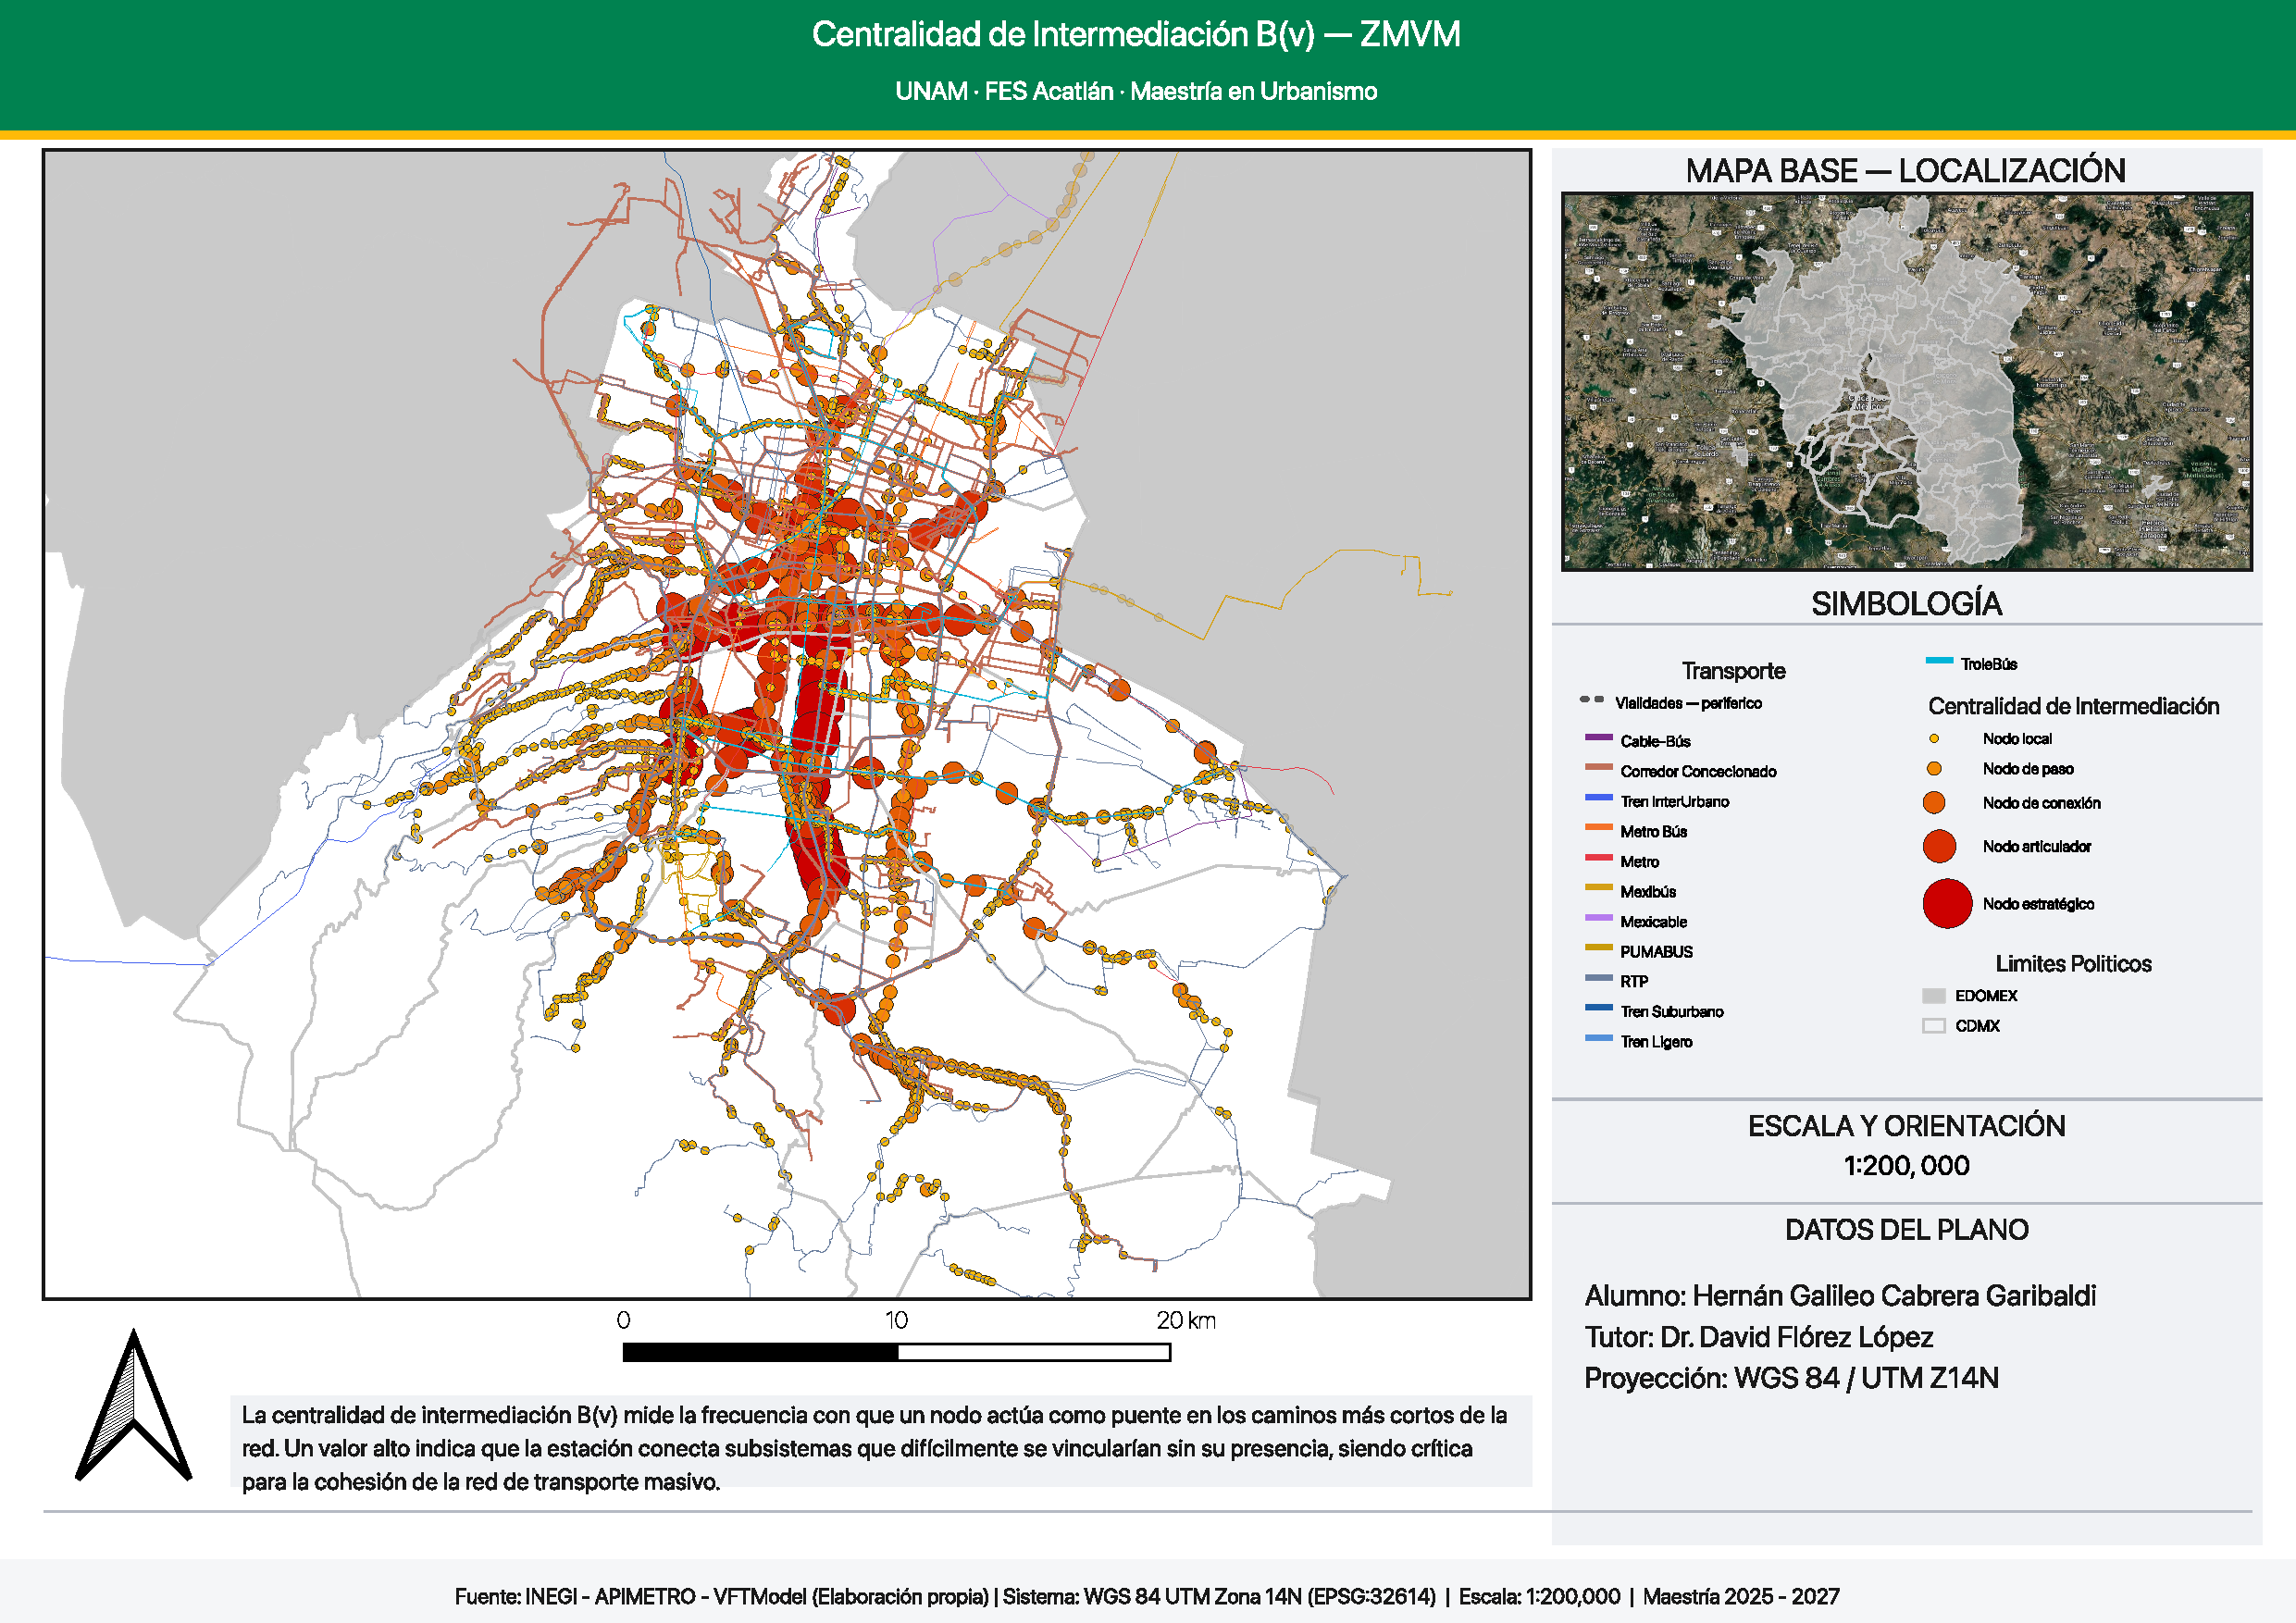
\includegraphics[width=\textwidth]{Figures/Mapas/Qgis_Resources/RedActual/Mapa_Betweenness}
  \caption[Centralidad de intermediación $B(v)$ — alta resolución]{Centralidad
  de intermediación normalizada $B(v)$ calculada sobre el grafo completo de
  10{,}561 nodos mediante el algoritmo de Brandes. Cada punto representa una
  estación; su tamaño y color indican la proporción de caminos mínimos de la red
  que pasan por ese nodo. Los valores más altos (puntos grandes en rojo o naranja)
  señalan los nodos cuya remoción tendría el mayor impacto sobre la conectividad
  global del sistema.}
  \label{fig:anx-f-qgis-betweenness}
  \fuentefigura{Elaboración propia con \textbf{Transport-gis-zmvm-mjg};
    datos: \gtfs{} \textsc{semovi} 2024 e \textsc{inegi} 2023.}
\end{figure}

% =============================================================================
\section{Tableros Apimetro — Tableau Desktop}
\label{anx:f-tableau-apimetro}
% =============================================================================

Los tableros de esta sección provienen del conector \textbf{WDC} de
\textbf{Transport-gis-zmvm-mjg}, que alimenta Tableau Desktop con los datos de
afluencia e infraestructura procesados por \textbf{Apimetro}.

% --- F.2.1 -------------------------------------------------------------------
\subsection{Dashboard: Red Metropolitana}
\label{anx:f-tab-api-dashboard}

\begin{figure}[p]
  \centering
  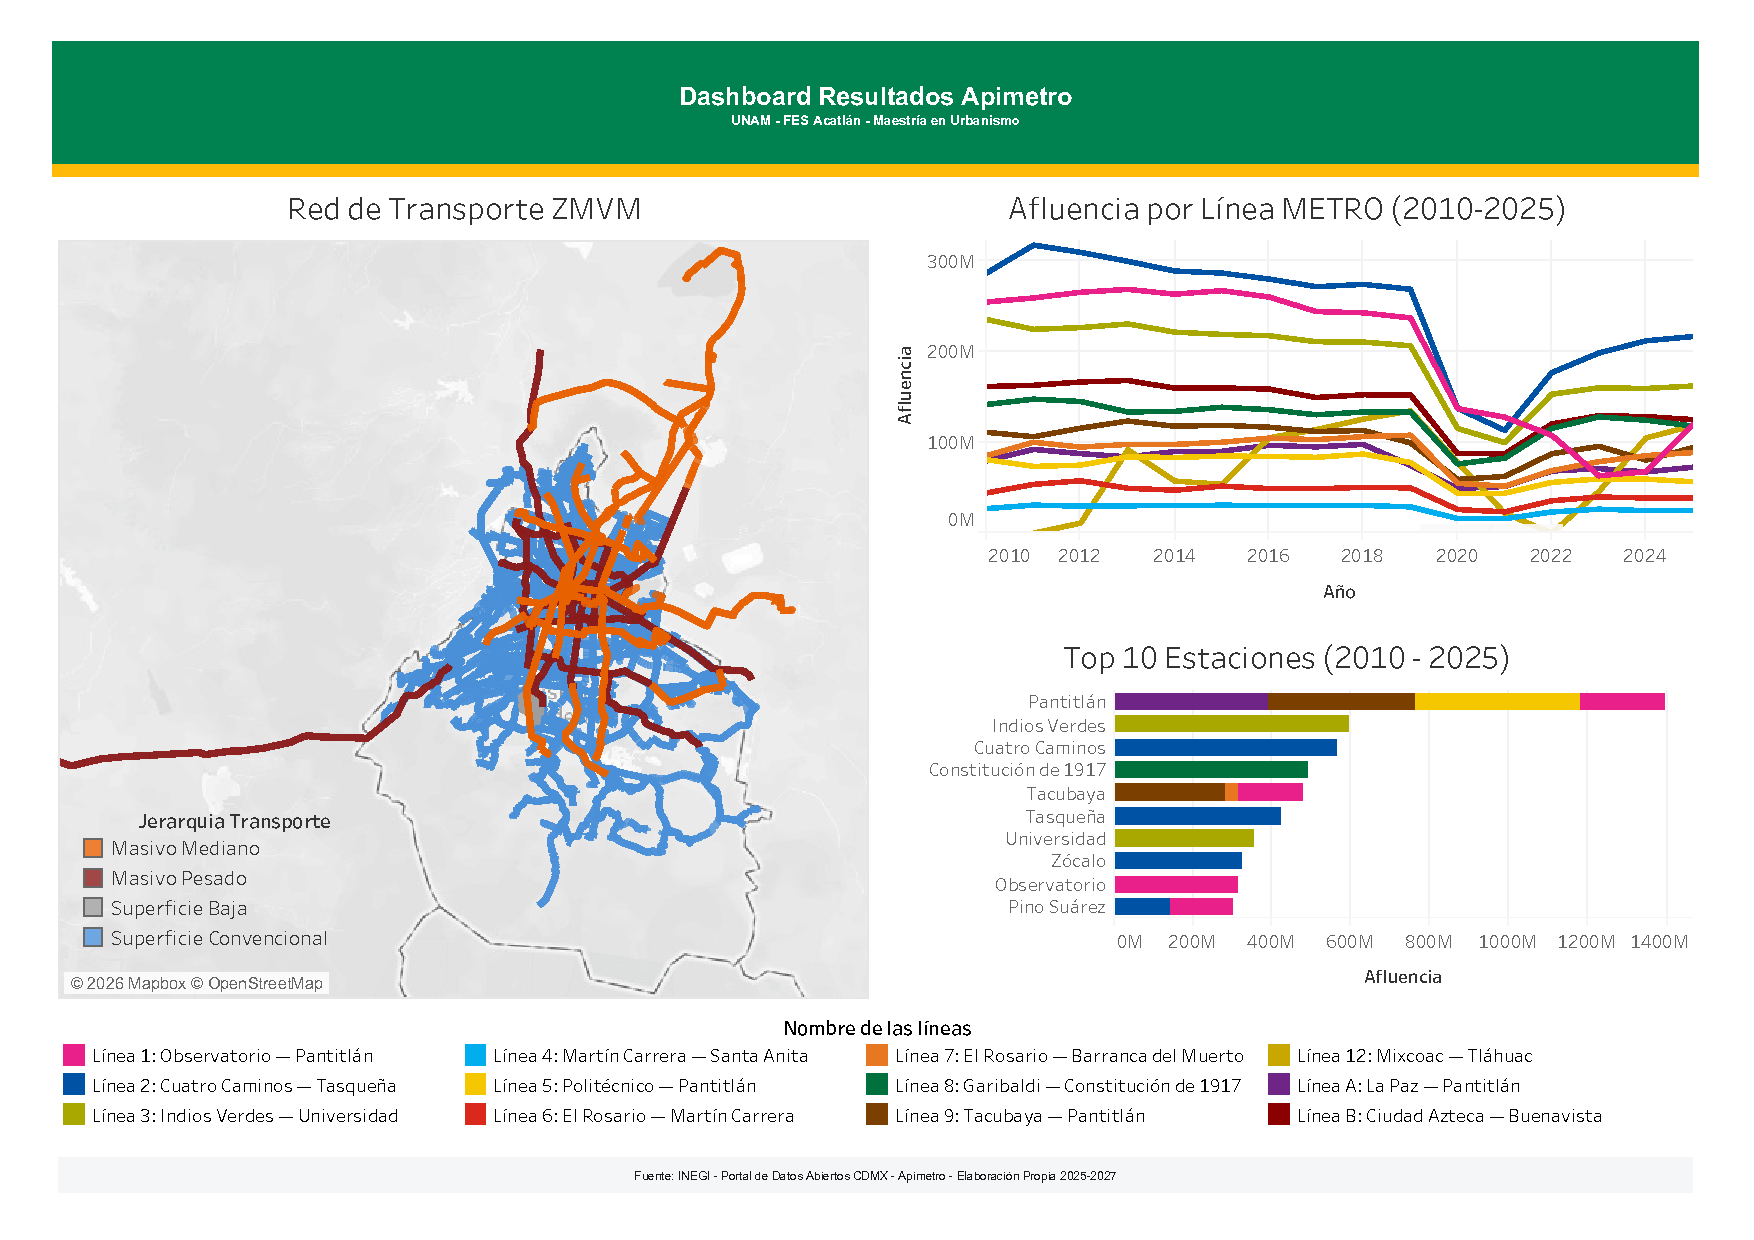
\includegraphics[width=\textwidth]{Figures/Mapas/Tableau_Resources/RedActual/Apimetro/Dashboards/Dashboard_Apimetro_2026}
  \caption[Dashboard Apimetro 2026 — red metropolitana completa]{Tablero de análisis
  de la red metropolitana construido sobre los datos de \textbf{Apimetro}. Integra
  en una sola vista: mapa georreferenciado de la red, distribución de afluencia por
  sistema y métricas de cobertura operativa de los doce sistemas de transporte de la
  \zmvm{}.}
  \label{fig:anx-f-tab-api-dashboard}
  \fuentefigura{Elaboración propia con \textbf{Tableau Desktop 2026.1};
    fuente de datos: \textbf{Apimetro} vía \textsc{wdc} Transport-gis.}
\end{figure}

% --- F.2.2 -------------------------------------------------------------------
\subsection{Dashboard: Red \zmvm{} — Vista Geográfica}
\label{anx:f-tab-api-red-zmvm}

\begin{figure}[p]
  \centering
  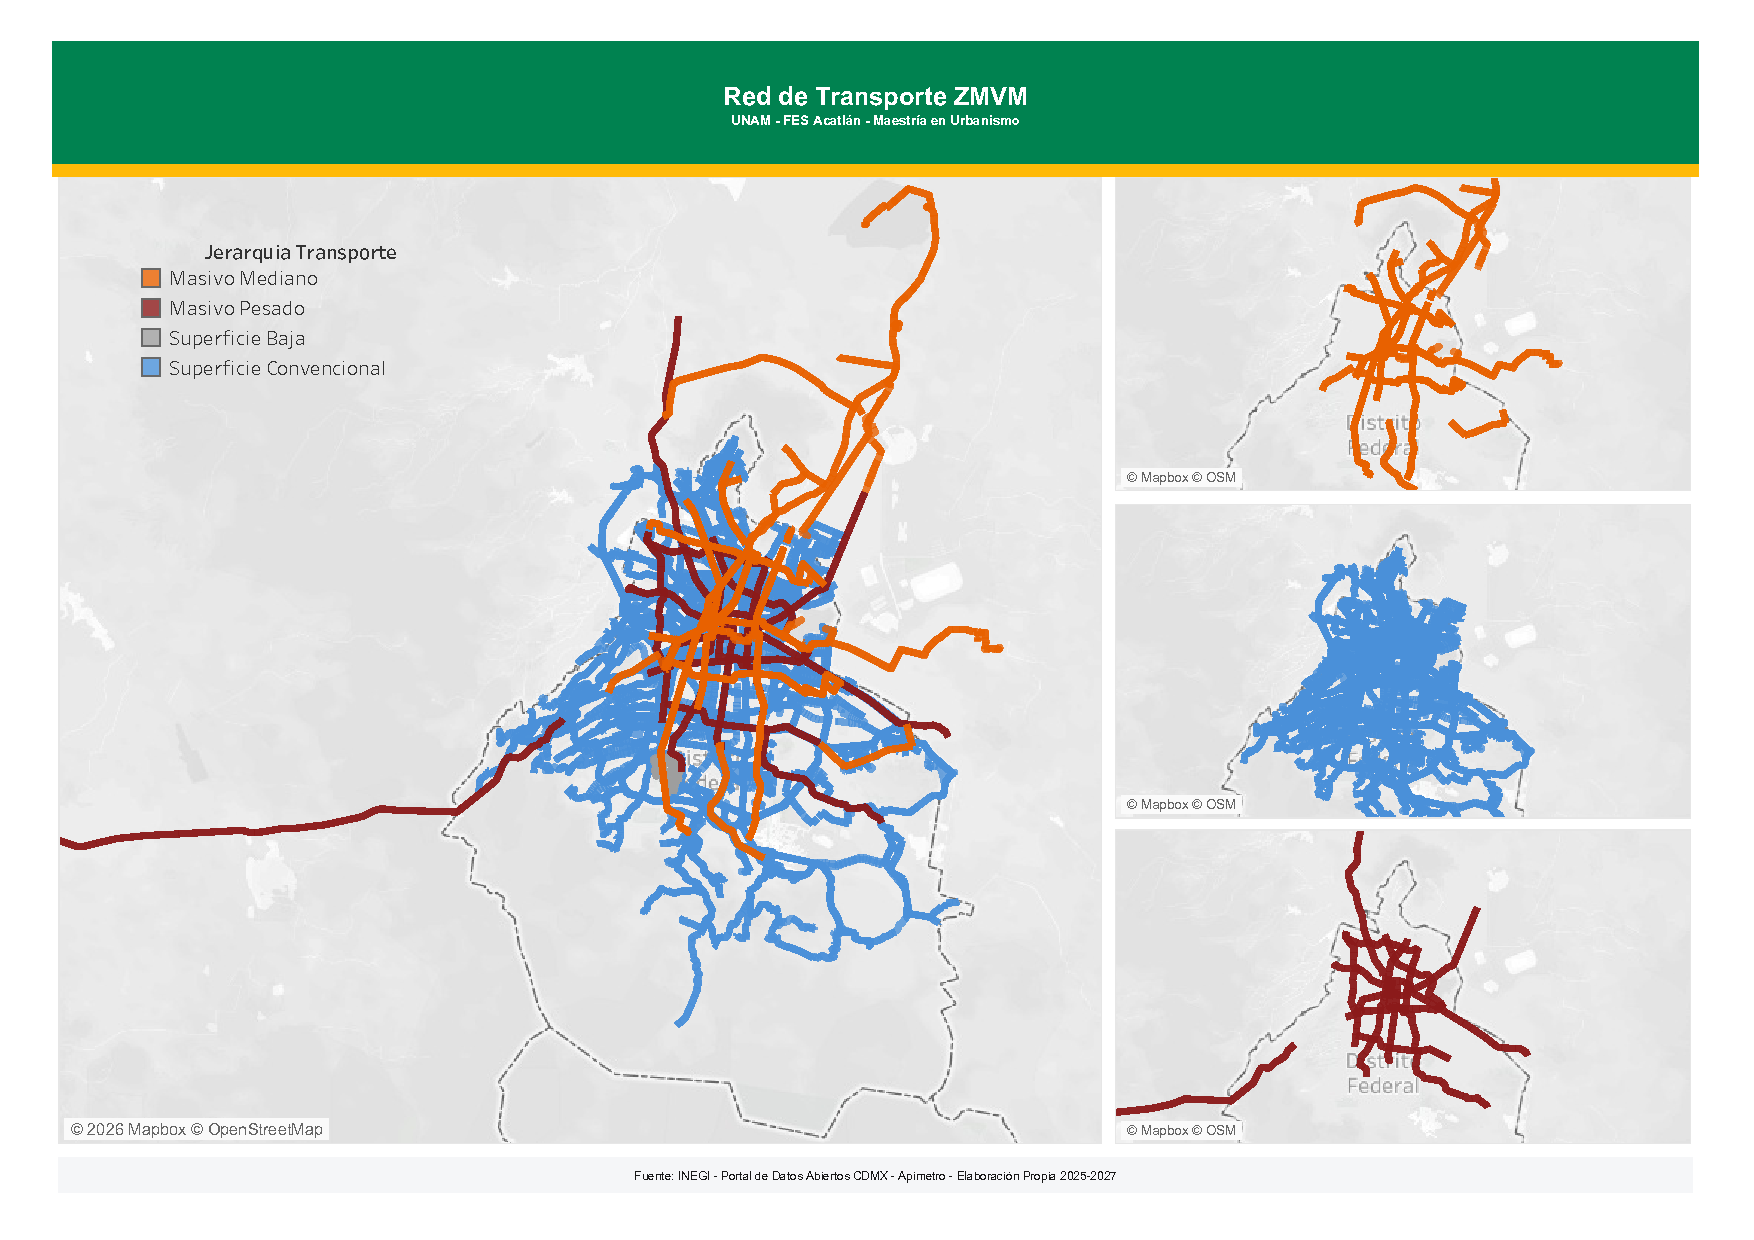
\includegraphics[width=\textwidth]{Figures/Mapas/Tableau_Resources/RedActual/Apimetro/Dashboards/Dashboard_Apimetro_2026_Red_ZMVM}
  \caption[Dashboard Apimetro 2026 — vista geográfica de la red]{Vista geográfica
  interactiva de la red de transporte de la \zmvm{} producida por Tableau Desktop
  a partir de los \textit{feeds} \gtfs{} normalizados por \textbf{Apimetro}.
  Cada línea representa una ruta operativa con su trazado espacial real.}
  \label{fig:anx-f-tab-api-red-zmvm}
  \fuentefigura{Elaboración propia con \textbf{Tableau Desktop 2026.1};
    fuente de datos: \textbf{Apimetro} vía \textsc{wdc} Transport-gis.}
\end{figure}

% --- F.2.3 -------------------------------------------------------------------
\subsection{Gráfica: Top~10 Estaciones por Afluencia}
\label{anx:f-tab-api-top10}

\begin{figure}[htb]
  \centering
  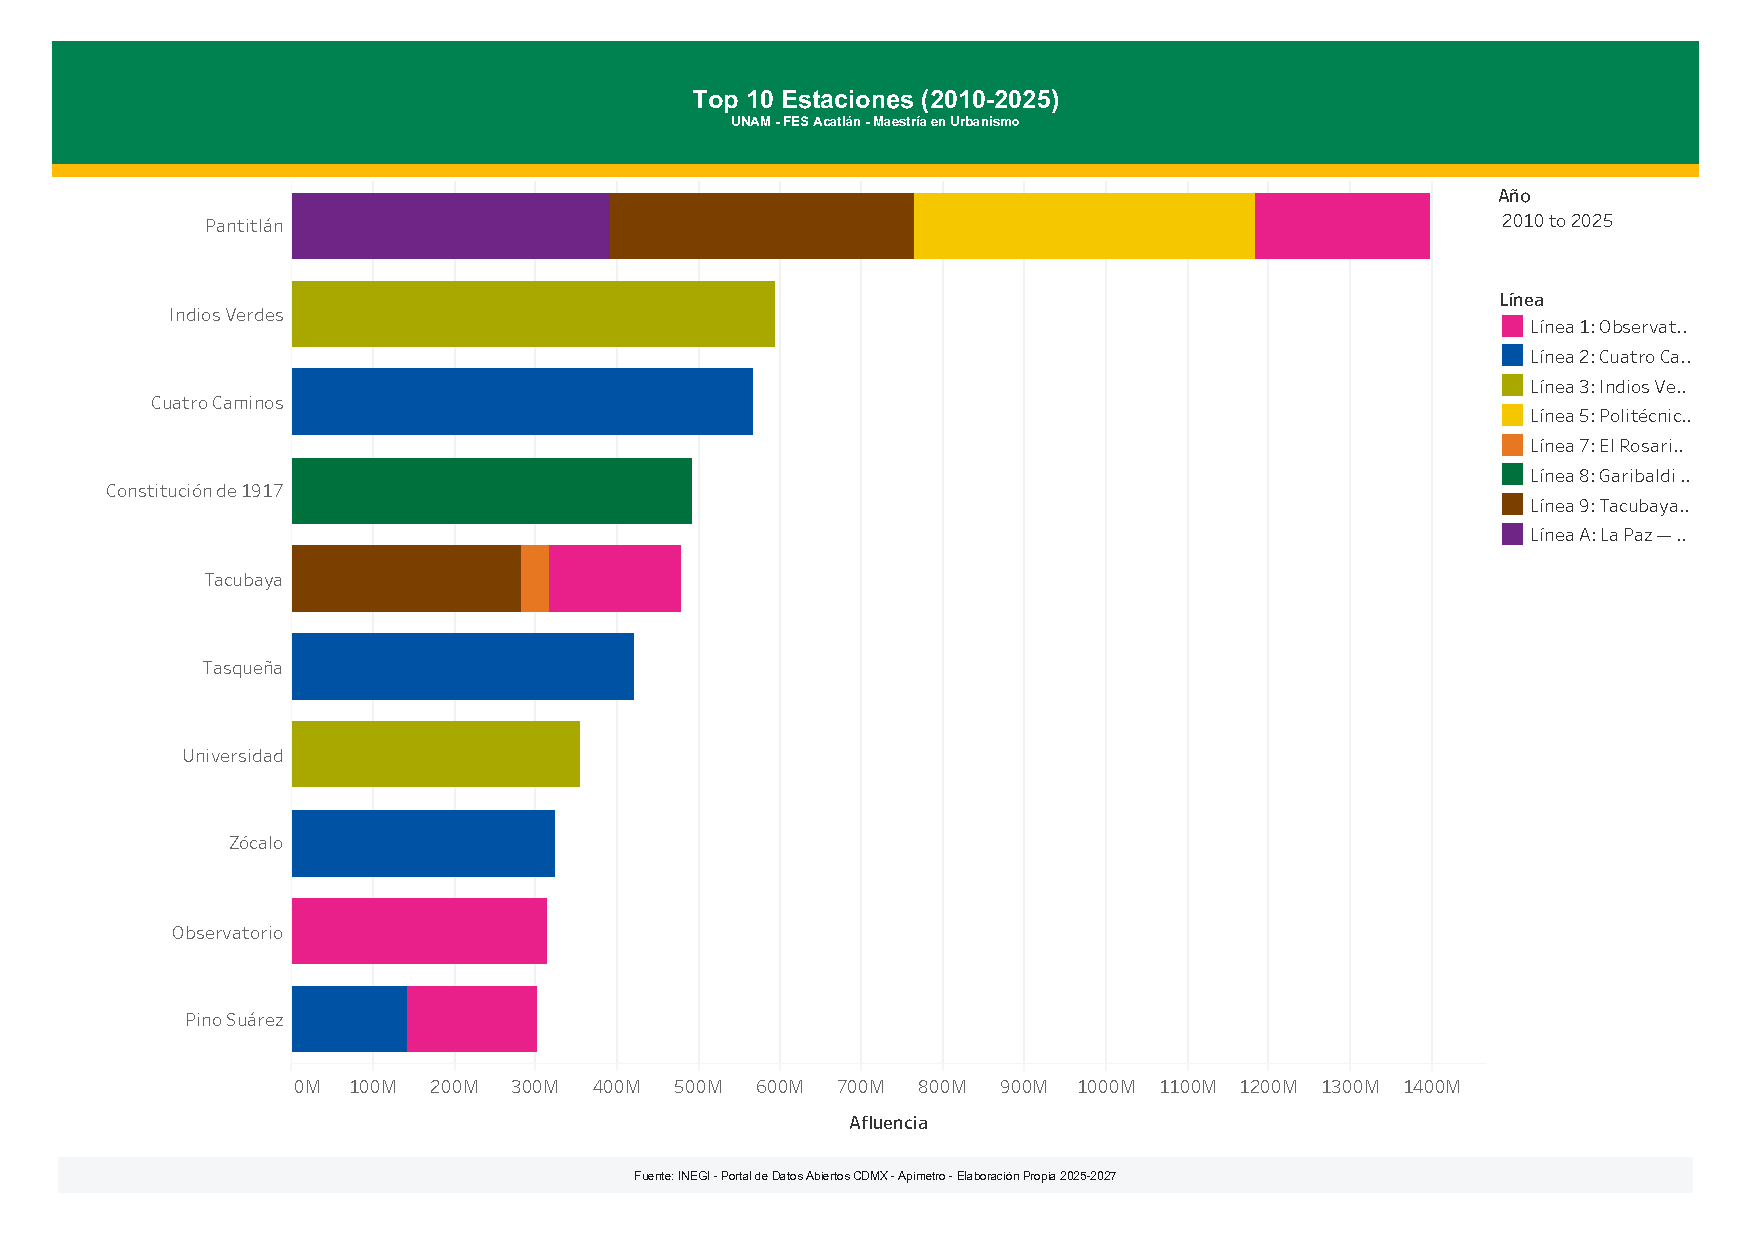
\includegraphics[width=0.9\textwidth]{Figures/Mapas/Tableau_Resources/RedActual/Apimetro/UniGrafica/Grafica_Apimetro_2026_Top_10_estaciones}
  \caption[Top~10 estaciones de la \zmvm{} por afluencia registrada]{Las diez
  estaciones con mayor afluencia anual registrada en los sistemas de transporte
  masivo de la \zmvm{}, según los datos operativos integrados por
  \textbf{Apimetro}. El indicador de afluencia sirve como proxy de demanda real
  para contextualizar los resultados de centralidad del Modelo VFT.}
  \label{fig:anx-f-tab-api-top10}
  \fuentefigura{Elaboración propia con \textbf{Tableau Desktop 2026.1};
    fuente de datos: \textbf{Apimetro} vía \textsc{wdc} Transport-gis.}
\end{figure}

% --- F.2.4 -------------------------------------------------------------------
\subsection{Gráfica: Afluencia Metro — Serie Anual}
\label{anx:f-tab-api-afluencia}

\begin{figure}[htb]
  \centering
  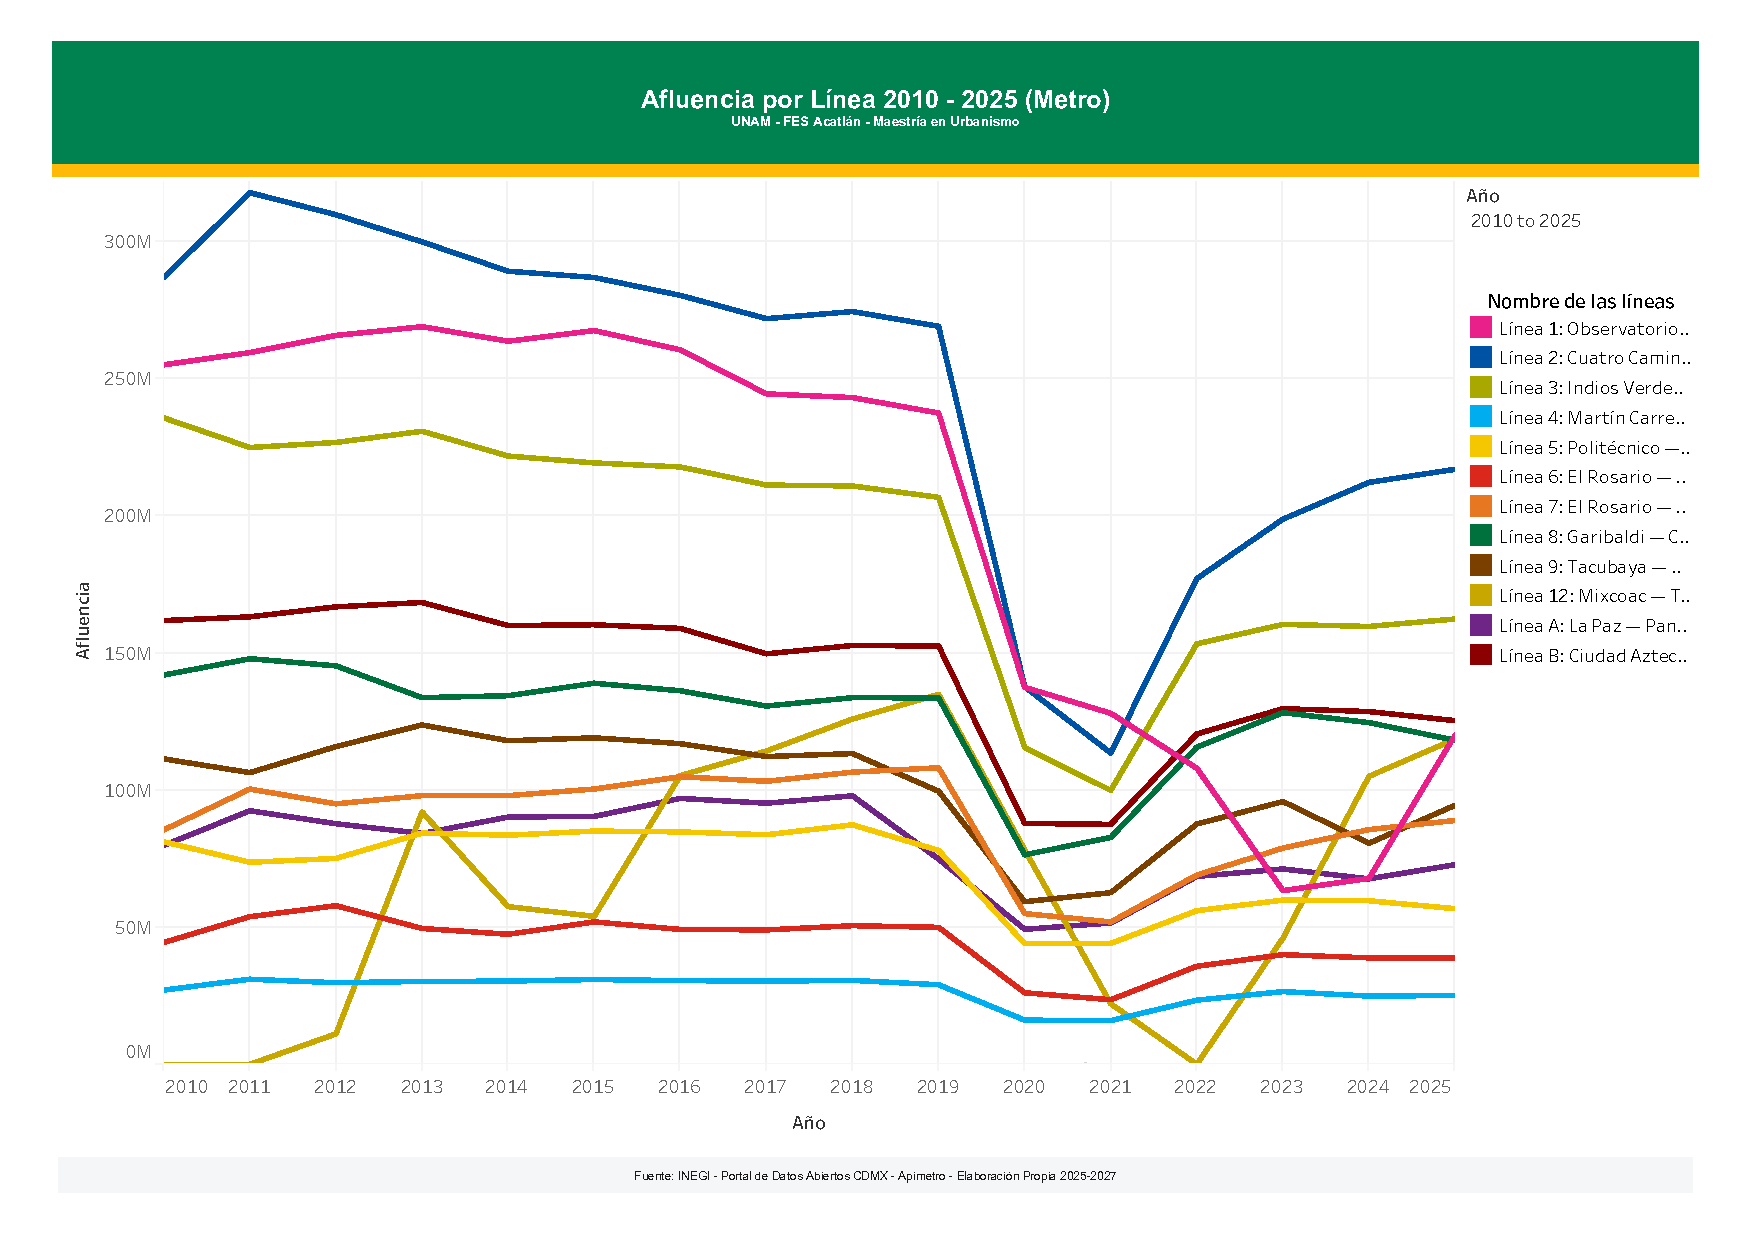
\includegraphics[width=0.9\textwidth]{Figures/Mapas/Tableau_Resources/RedActual/Apimetro/UniGrafica/Grafica_Apimetro_2026_Afluencia_Metro_Anual}
  \caption[Afluencia anual del Sistema de Transporte Colectivo Metro]{Serie
  histórica de afluencia anual del Sistema de Transporte Colectivo Metro de la
  \cdmx{}, según los registros integrados en \textbf{Apimetro}. Referencia de
  contexto para interpretar la centralidad de las estaciones del Metro en los
  resultados del indicador $B(v)$.}
  \label{fig:anx-f-tab-api-afluencia}
  \fuentefigura{Elaboración propia con \textbf{Tableau Desktop 2026.1};
    fuente de datos: \textbf{Apimetro} vía \textsc{wdc} Transport-gis.}
\end{figure}

% --- F.2.5 -------------------------------------------------------------------
\subsection{Gráfica: Calidad del Servicio por Sistema}
\label{anx:f-tab-api-calidad}

\begin{figure}[htb]
  \centering
  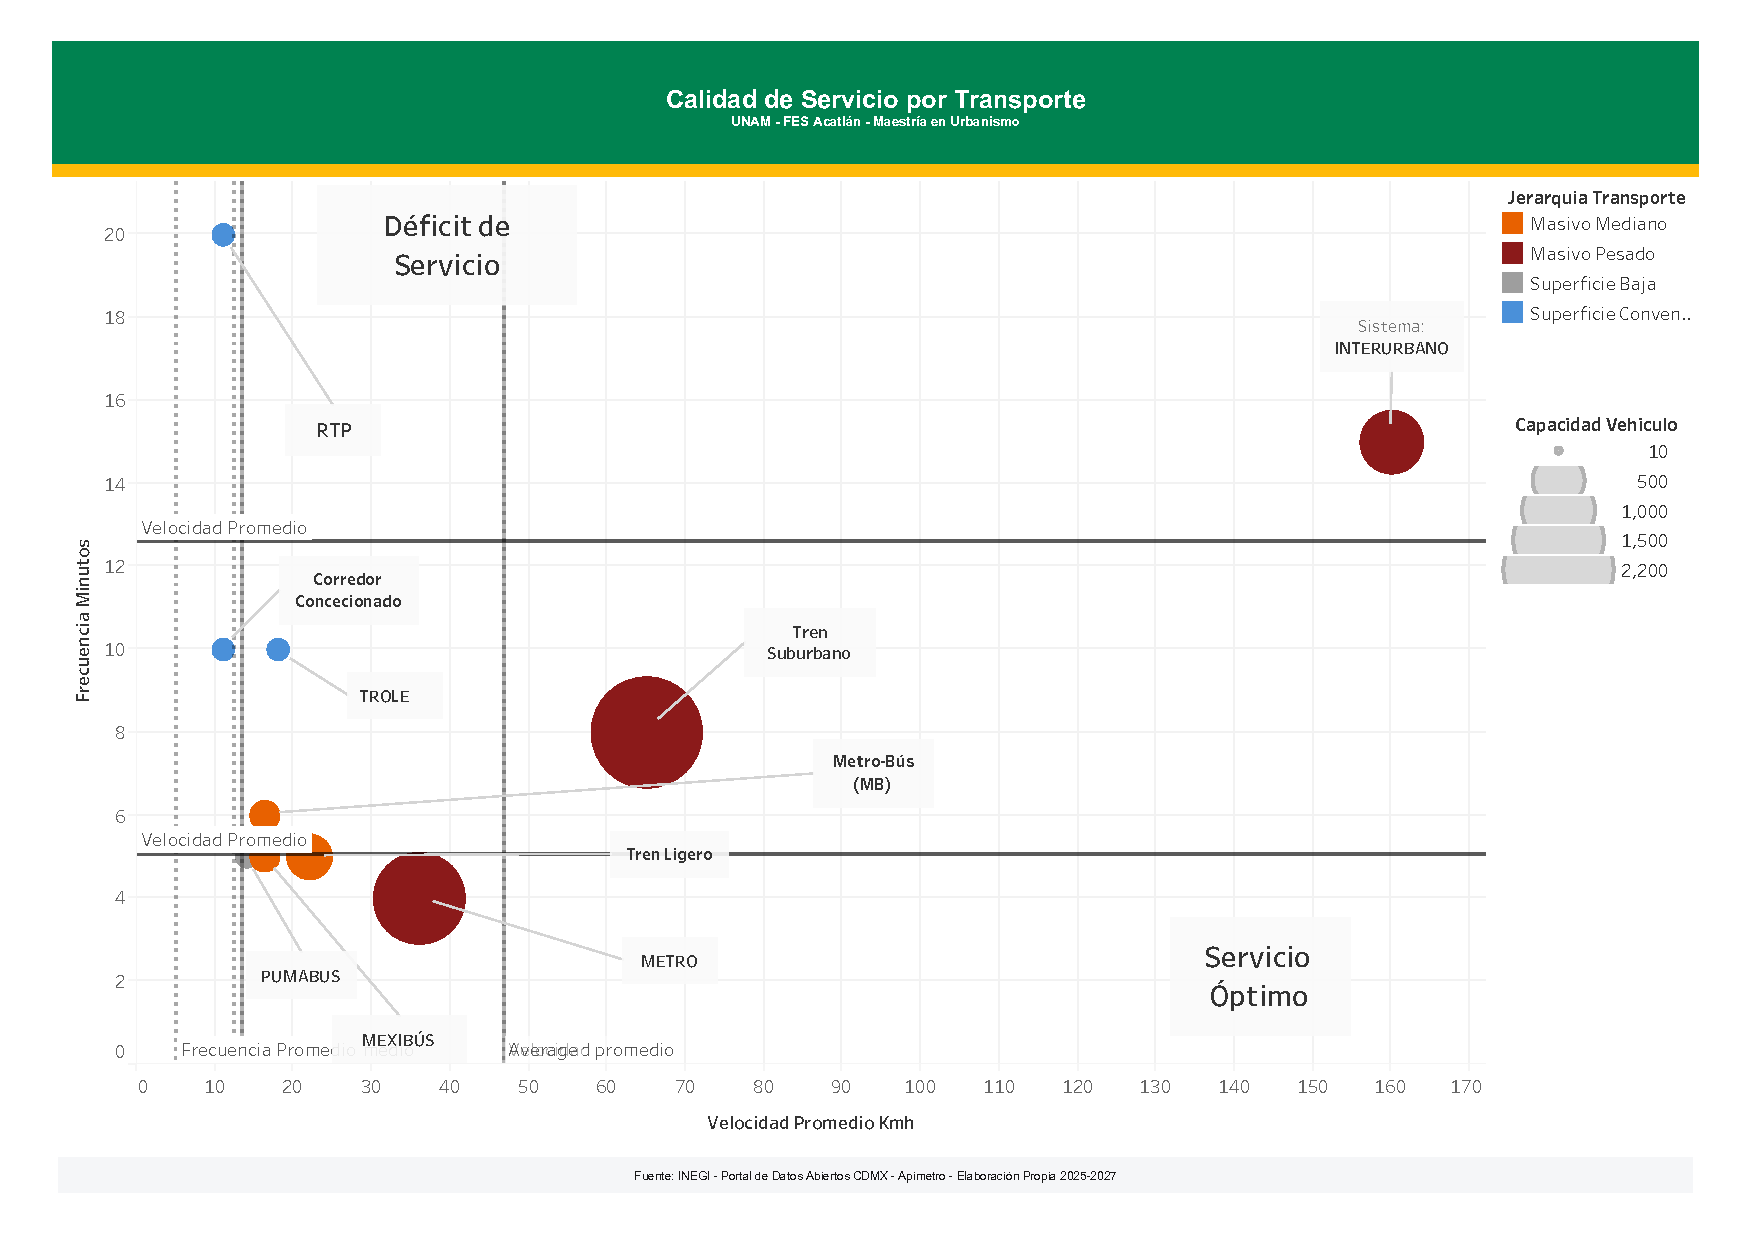
\includegraphics[width=0.9\textwidth]{Figures/Mapas/Tableau_Resources/RedActual/Apimetro/UniGrafica/Grafica_Dashboard_Apimetro_2026_Calidad_Servicio}
  \caption[Indicadores de calidad del servicio por sistema de transporte]{Comparación
  de indicadores de calidad del servicio (frecuencia, velocidad comercial, cobertura
  horaria) entre los doce sistemas de transporte de la \zmvm{}, según los atributos
  operativos registrados en \textbf{Apimetro}.}
  \label{fig:anx-f-tab-api-calidad}
  \fuentefigura{Elaboración propia con \textbf{Tableau Desktop 2026.1};
    fuente de datos: \textbf{Apimetro} vía \textsc{wdc} Transport-gis.}
\end{figure}

% =============================================================================
\section{Tableros Modelo VFT — Tableau Desktop}
\label{anx:f-tableau-vftmodel}
% =============================================================================

Los tableros de esta sección consumen los resultados del \textbf{Modelo VFT}
exportados como \textit{GeoPackages} y servidos a Tableau Desktop a través del
\textsc{api} \textbf{GeoProxy} de Transport-gis-zmvm-mjg.

% --- F.3.1 -------------------------------------------------------------------
\subsection{Dashboard: Fuerza Capilar}
\label{anx:f-tab-vft-dashboard-fc}

\begin{figure}[p]
  \centering
  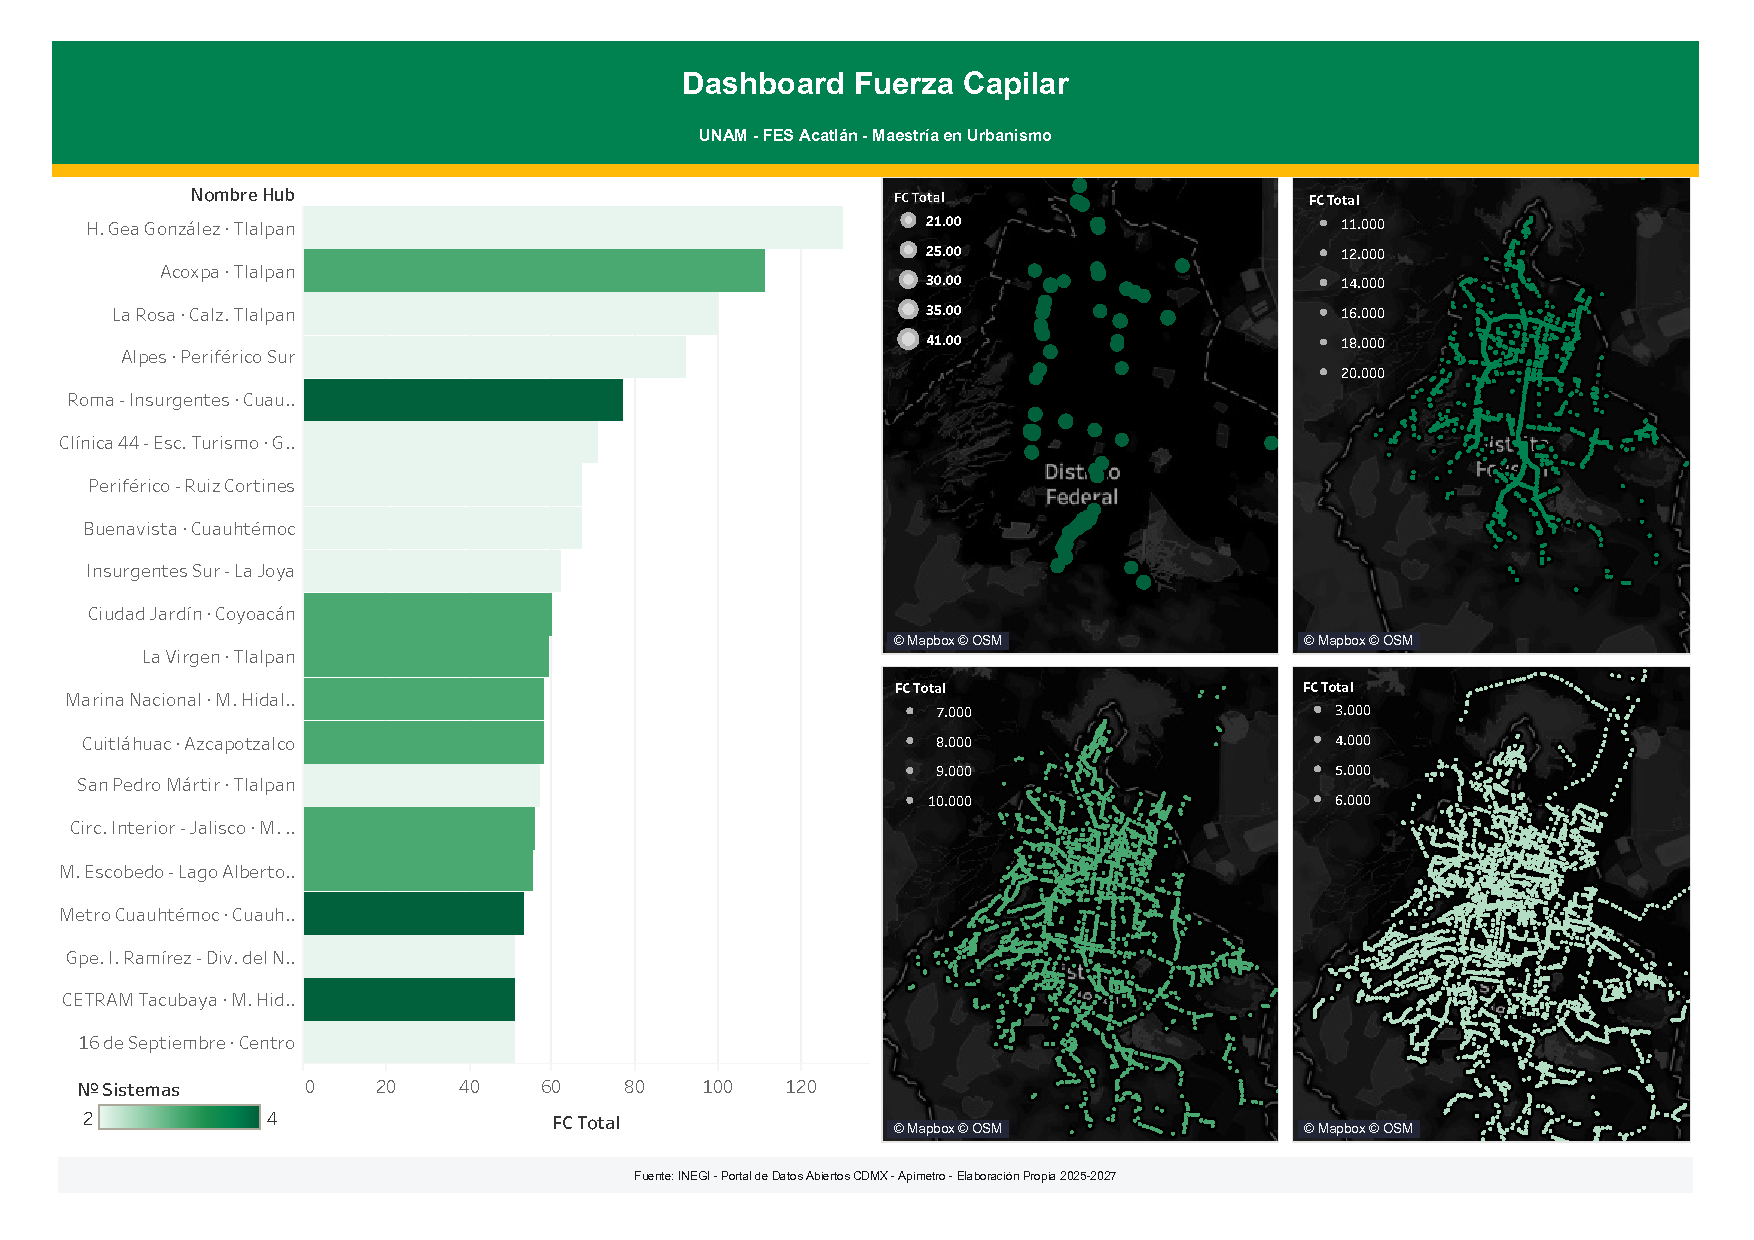
\includegraphics[width=\textwidth]{Figures/Mapas/Tableau_Resources/RedActual/VFTModel/Dashboards/Dashboard_VFTModel_2026_Fuerza_Capilar}
  \caption[Dashboard Modelo VFT 2026 — Fuerza Capilar $FC_h$]{Tablero de análisis
  del indicador de Fuerza Capilar $FC_h$. Combina la distribución espacial de los
  macrohubs (mapa), el histograma de la distribución del indicador y el ranking de
  los veinte nodos con mayor valor de $FC_h$ en la red de la \zmvm{}.}
  \label{fig:anx-f-tab-vft-dashboard-fc}
  \fuentefigura{Elaboración propia con \textbf{Tableau Desktop 2026.1};
    fuente de datos: \textbf{VFTModel} vía \textsc{api} GeoProxy.}
\end{figure}

% --- F.3.2 -------------------------------------------------------------------
\subsection{Dashboard: Factor de Desviación}
\label{anx:f-tab-vft-dashboard-df}

\begin{figure}[p]
  \centering
  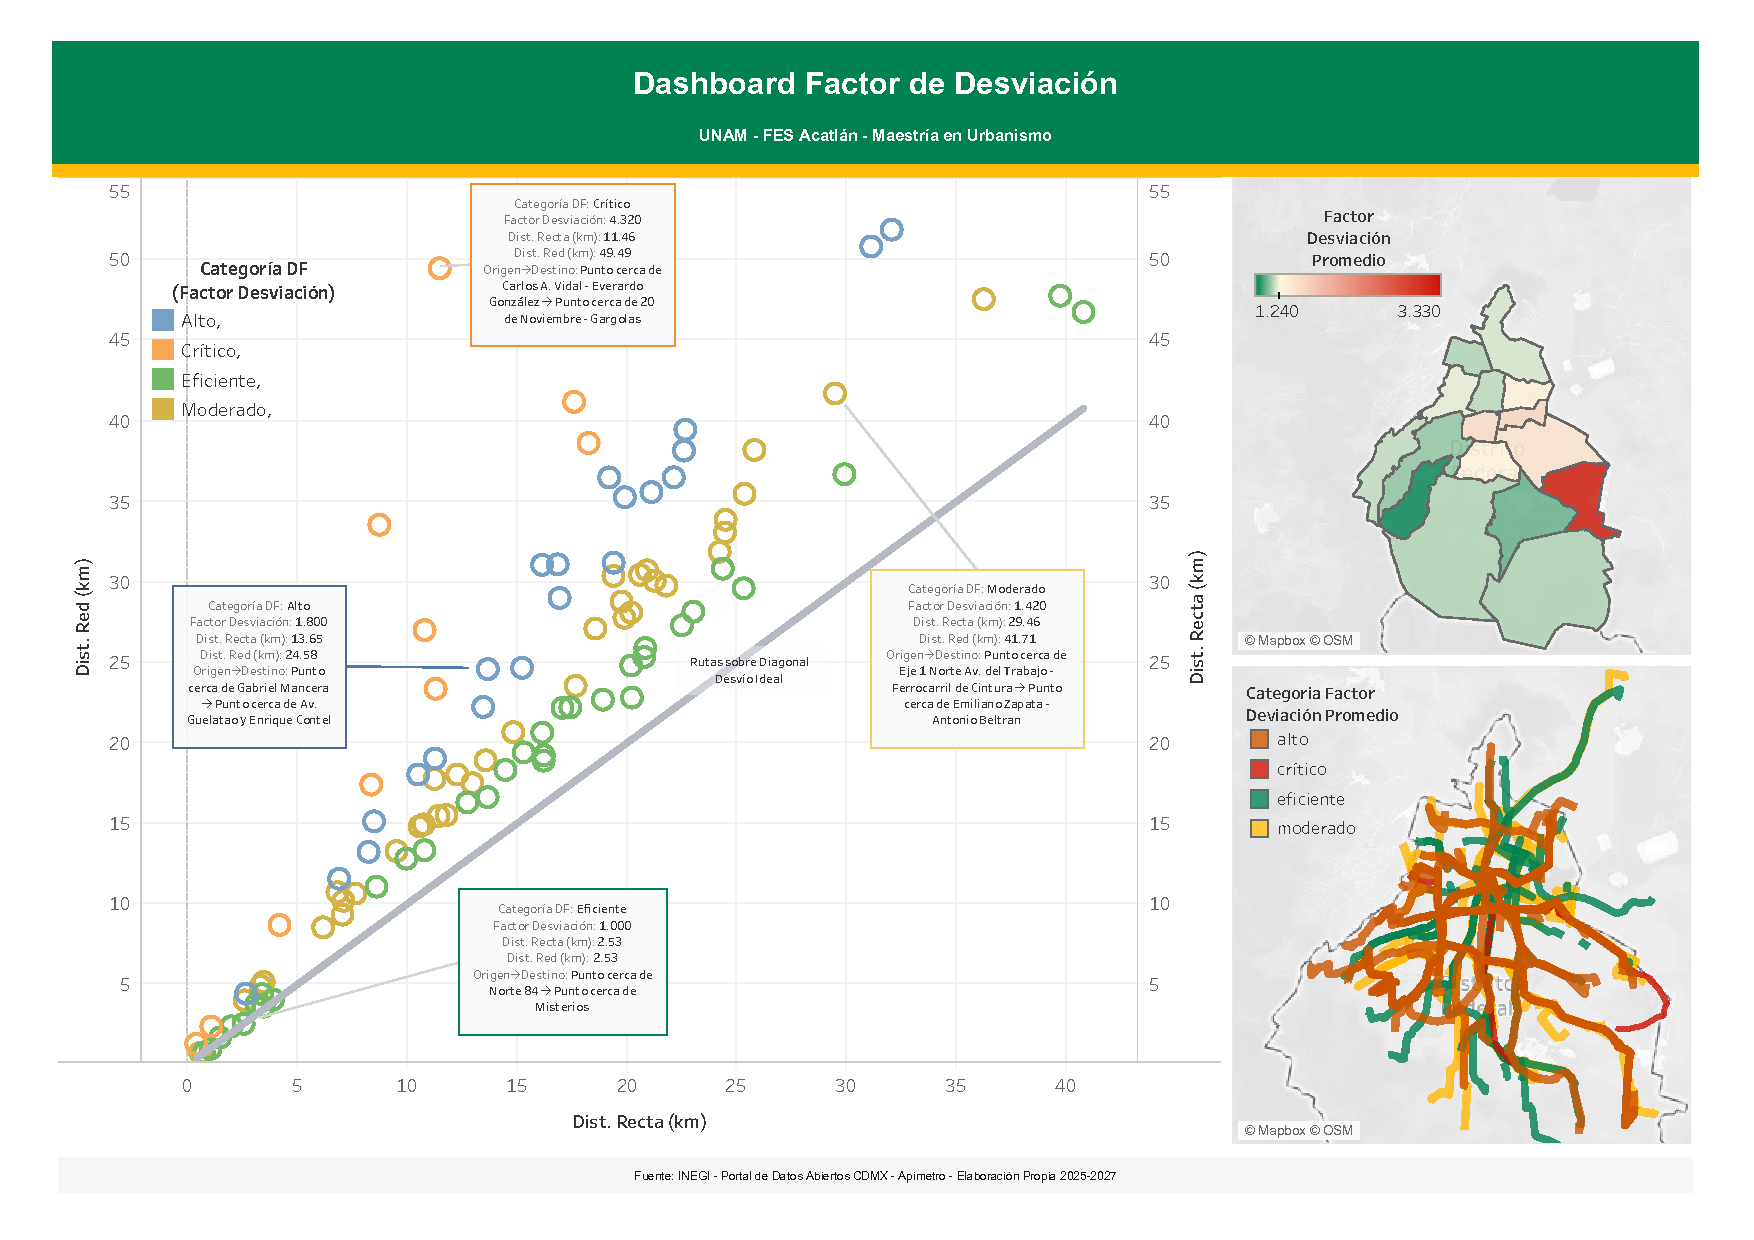
\includegraphics[width=\textwidth]{Figures/Mapas/Tableau_Resources/RedActual/VFTModel/Dashboards/Dashboard_VFTModel_2026_Factor_desviacion}
  \caption[Dashboard Modelo VFT 2026 — Factor de desviación $DI$]{Tablero de análisis
  del indicador de Factor de Desviación $DI$. Presenta la distribución espacial de
  los valores de $DI$ sobre la muestra de 100 rutas, el mapa de las zonas con mayor
  ineficiencia de trazado y la comparación por alcaldía y municipio.}
  \label{fig:anx-f-tab-vft-dashboard-df}
  \fuentefigura{Elaboración propia con \textbf{Tableau Desktop 2026.1};
    fuente de datos: \textbf{VFTModel} vía \textsc{api} GeoProxy.}
\end{figure}

% --- F.3.3 -------------------------------------------------------------------
\subsection{Dashboard: Centralidad de Intermediación}
\label{anx:f-tab-vft-dashboard-bv}

\begin{figure}[p]
  \centering
  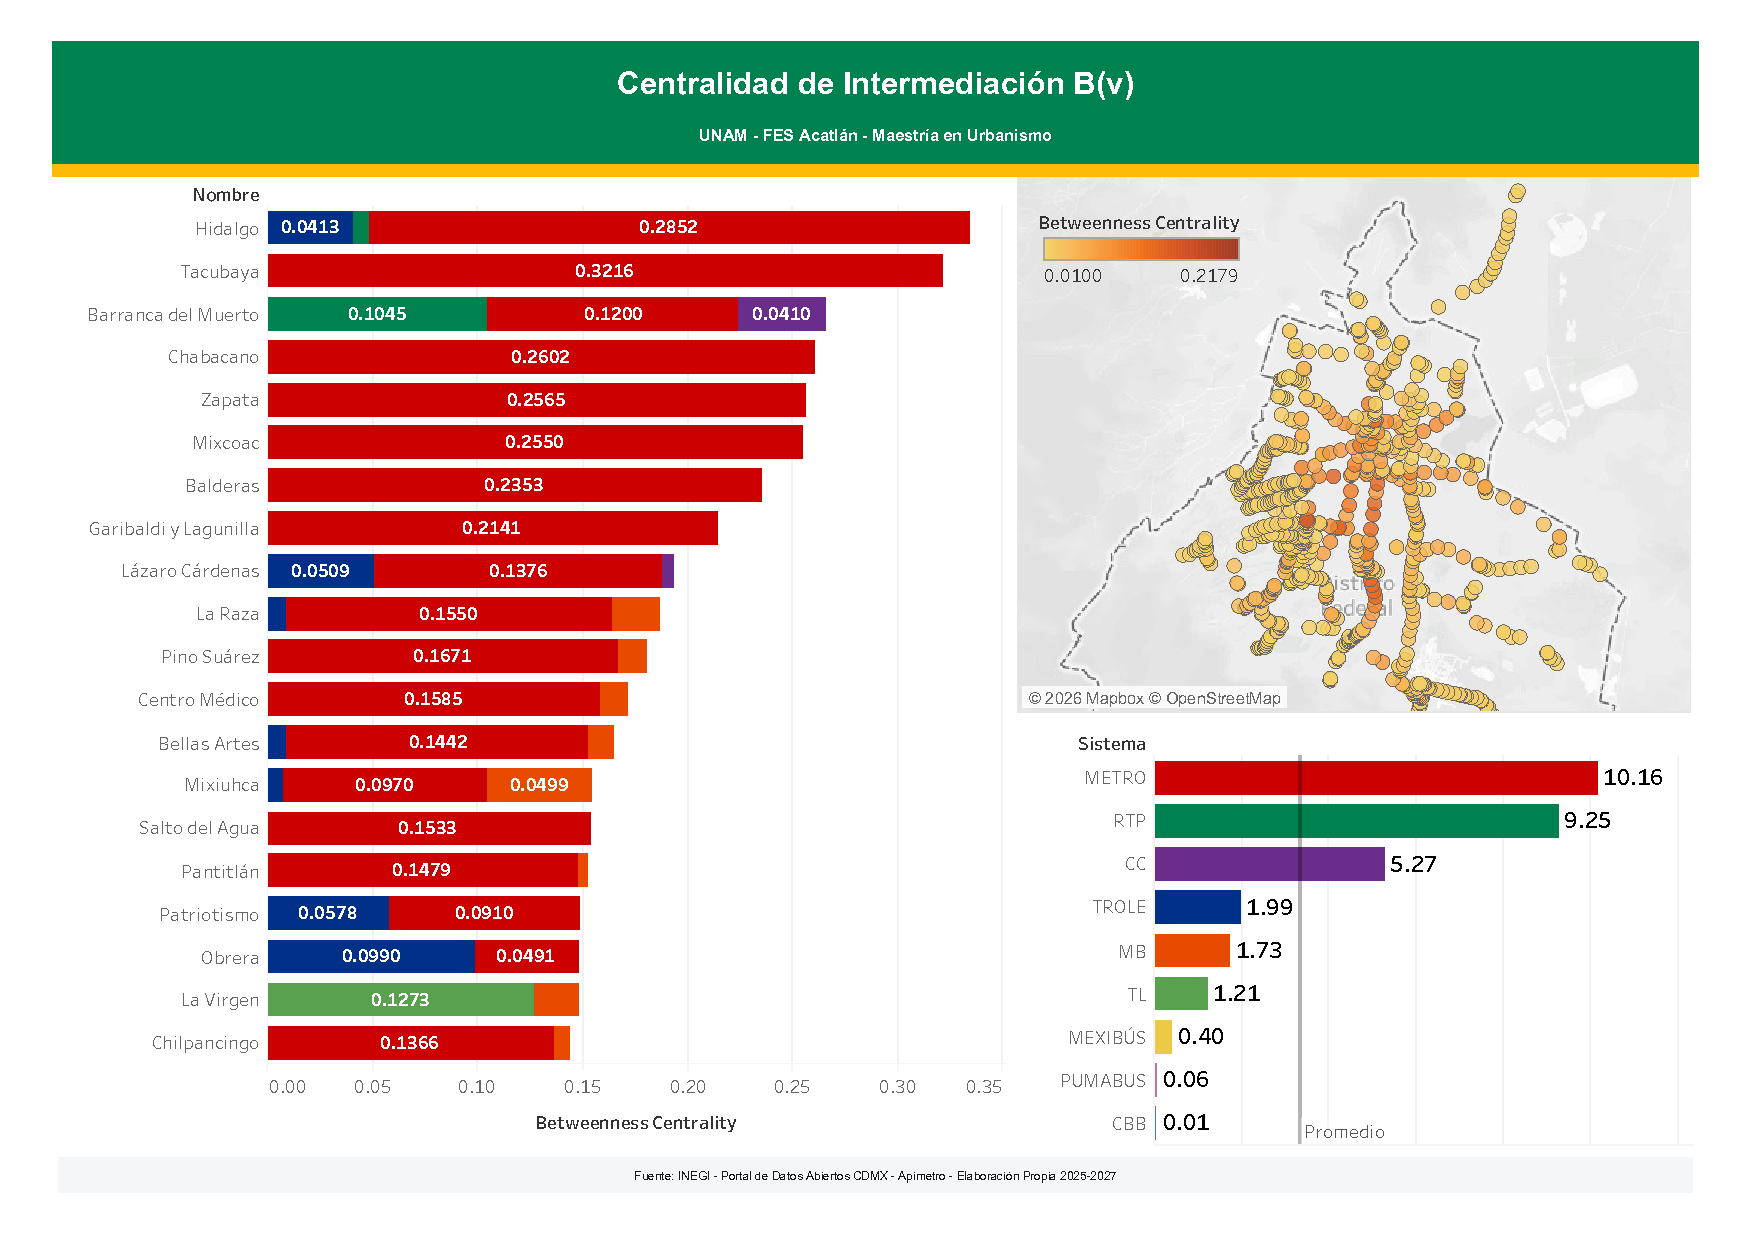
\includegraphics[width=\textwidth]{Figures/Mapas/Tableau_Resources/RedActual/VFTModel/Dashboards/Dashboard_VFTModel_2026_Centralidad_intermediacion}
  \caption[Dashboard Modelo VFT 2026 — Centralidad de intermediación $B(v)$]{Tablero
  de análisis del indicador $B(v)$. Integra el mapa de centralidad georreferenciado,
  el ranking de las estaciones con mayor valor de intermediación y la distribución
  por sistema de transporte. Los resultados corresponden a la corrida del
  2026-09-02 sobre los 10{,}561 nodos de la componente gigante del grafo.}
  \label{fig:anx-f-tab-vft-dashboard-bv}
  \fuentefigura{Elaboración propia con \textbf{Tableau Desktop 2026.1};
    fuente de datos: \textbf{VFTModel} vía \textsc{api} GeoProxy.}
\end{figure}

% --- F.3.4 -------------------------------------------------------------------
\subsection{Gráfica: Cobertura por Sistema de Transporte}
\label{anx:f-tab-vft-cobertura-sistema}

\begin{figure}[htb]
  \centering
  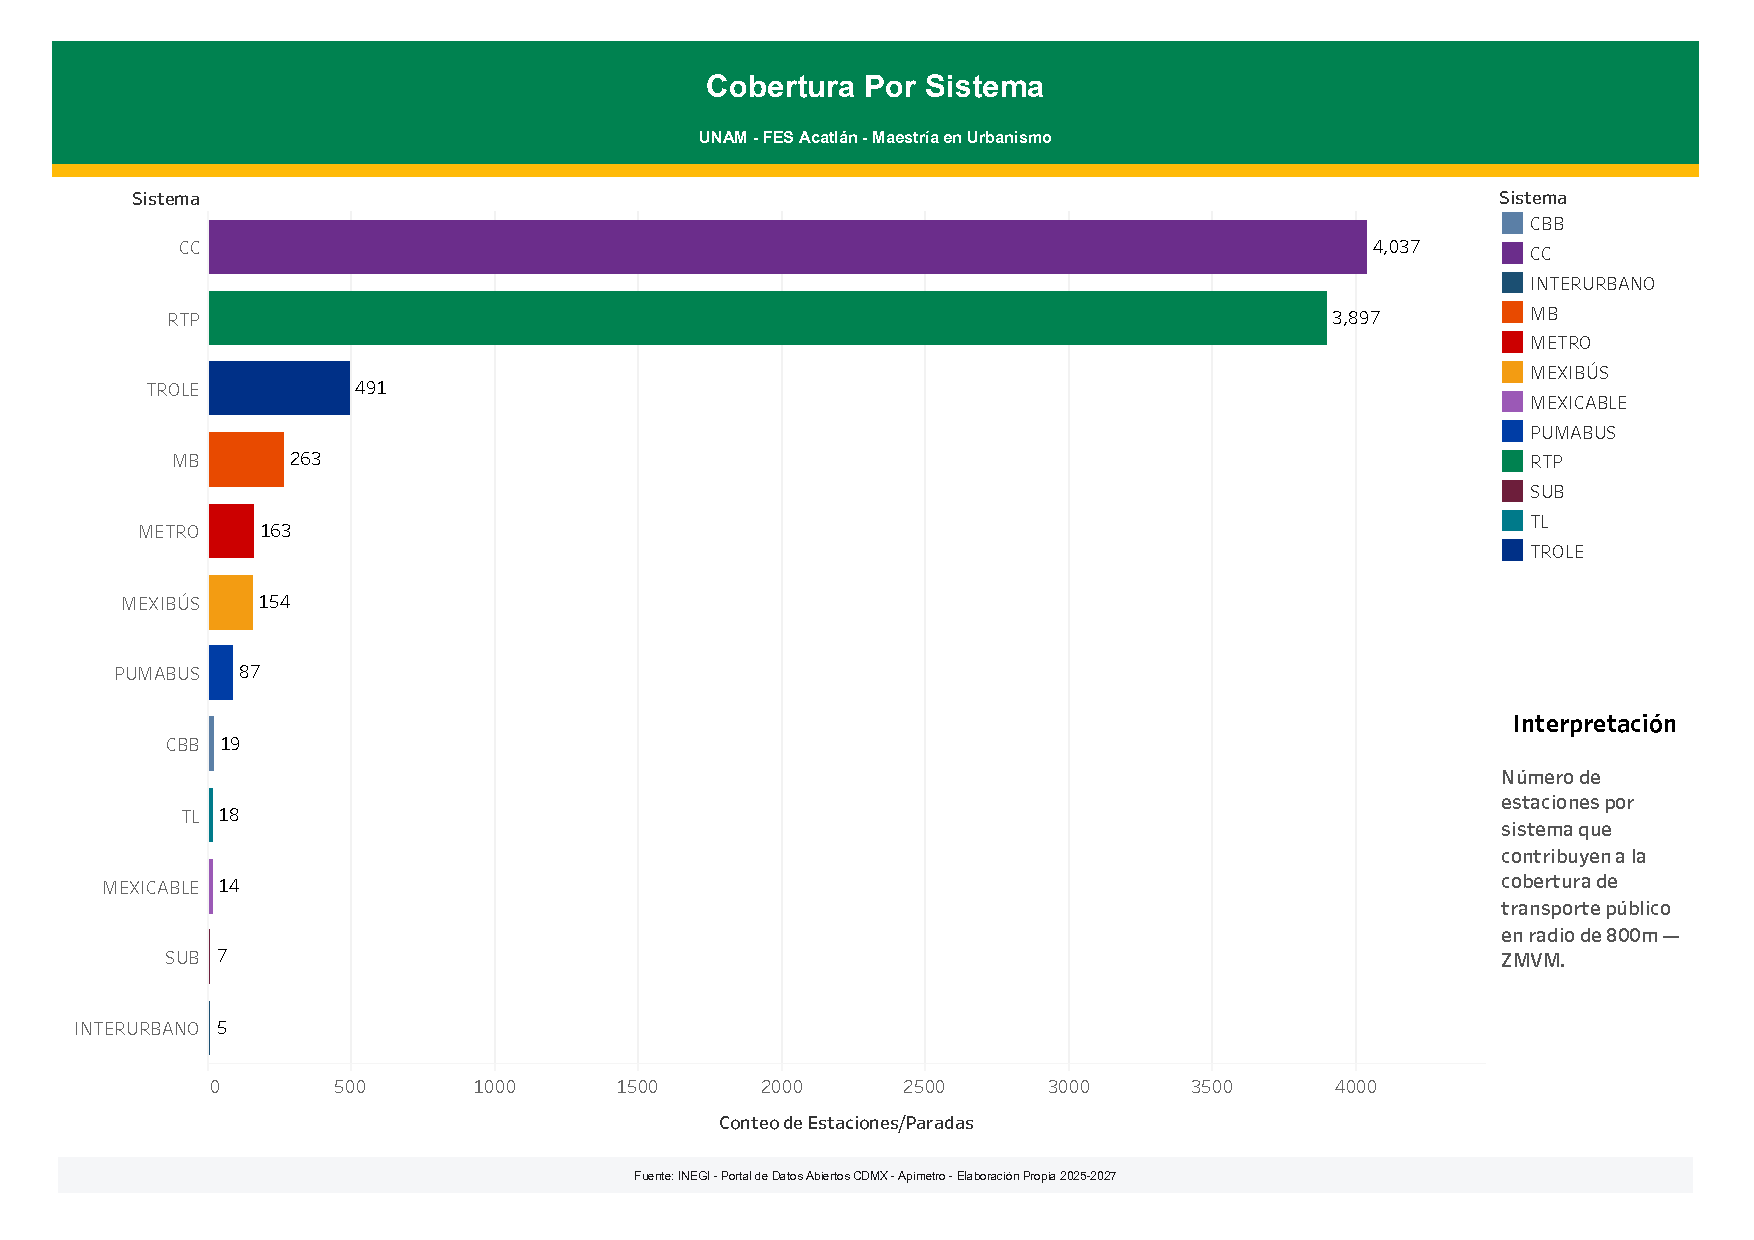
\includegraphics[width=0.9\textwidth]{Figures/Mapas/Tableau_Resources/RedActual/VFTModel/UniGrafica/Grafica_VFTModel_2026_Cobertura_sistema}
  \caption[Nivel de cobertura $C$ por sistema de transporte]{Comparación del nivel
  de cobertura espacial $C$ entre los doce sistemas de transporte de la \zmvm{},
  medido como porcentaje del área metropolitana alcanzable a 800~m de caminata
  desde las paradas de cada sistema.}
  \label{fig:anx-f-tab-vft-cobertura-sistema}
  \fuentefigura{Elaboración propia con \textbf{Tableau Desktop 2026.1};
    fuente de datos: \textbf{VFTModel} vía \textsc{api} GeoProxy.}
\end{figure}

% --- F.3.5 -------------------------------------------------------------------
\subsection{Gráfica: Cobertura por Alcaldía}
\label{anx:f-tab-vft-cobertura-alcaldia}

\begin{figure}[htb]
  \centering
  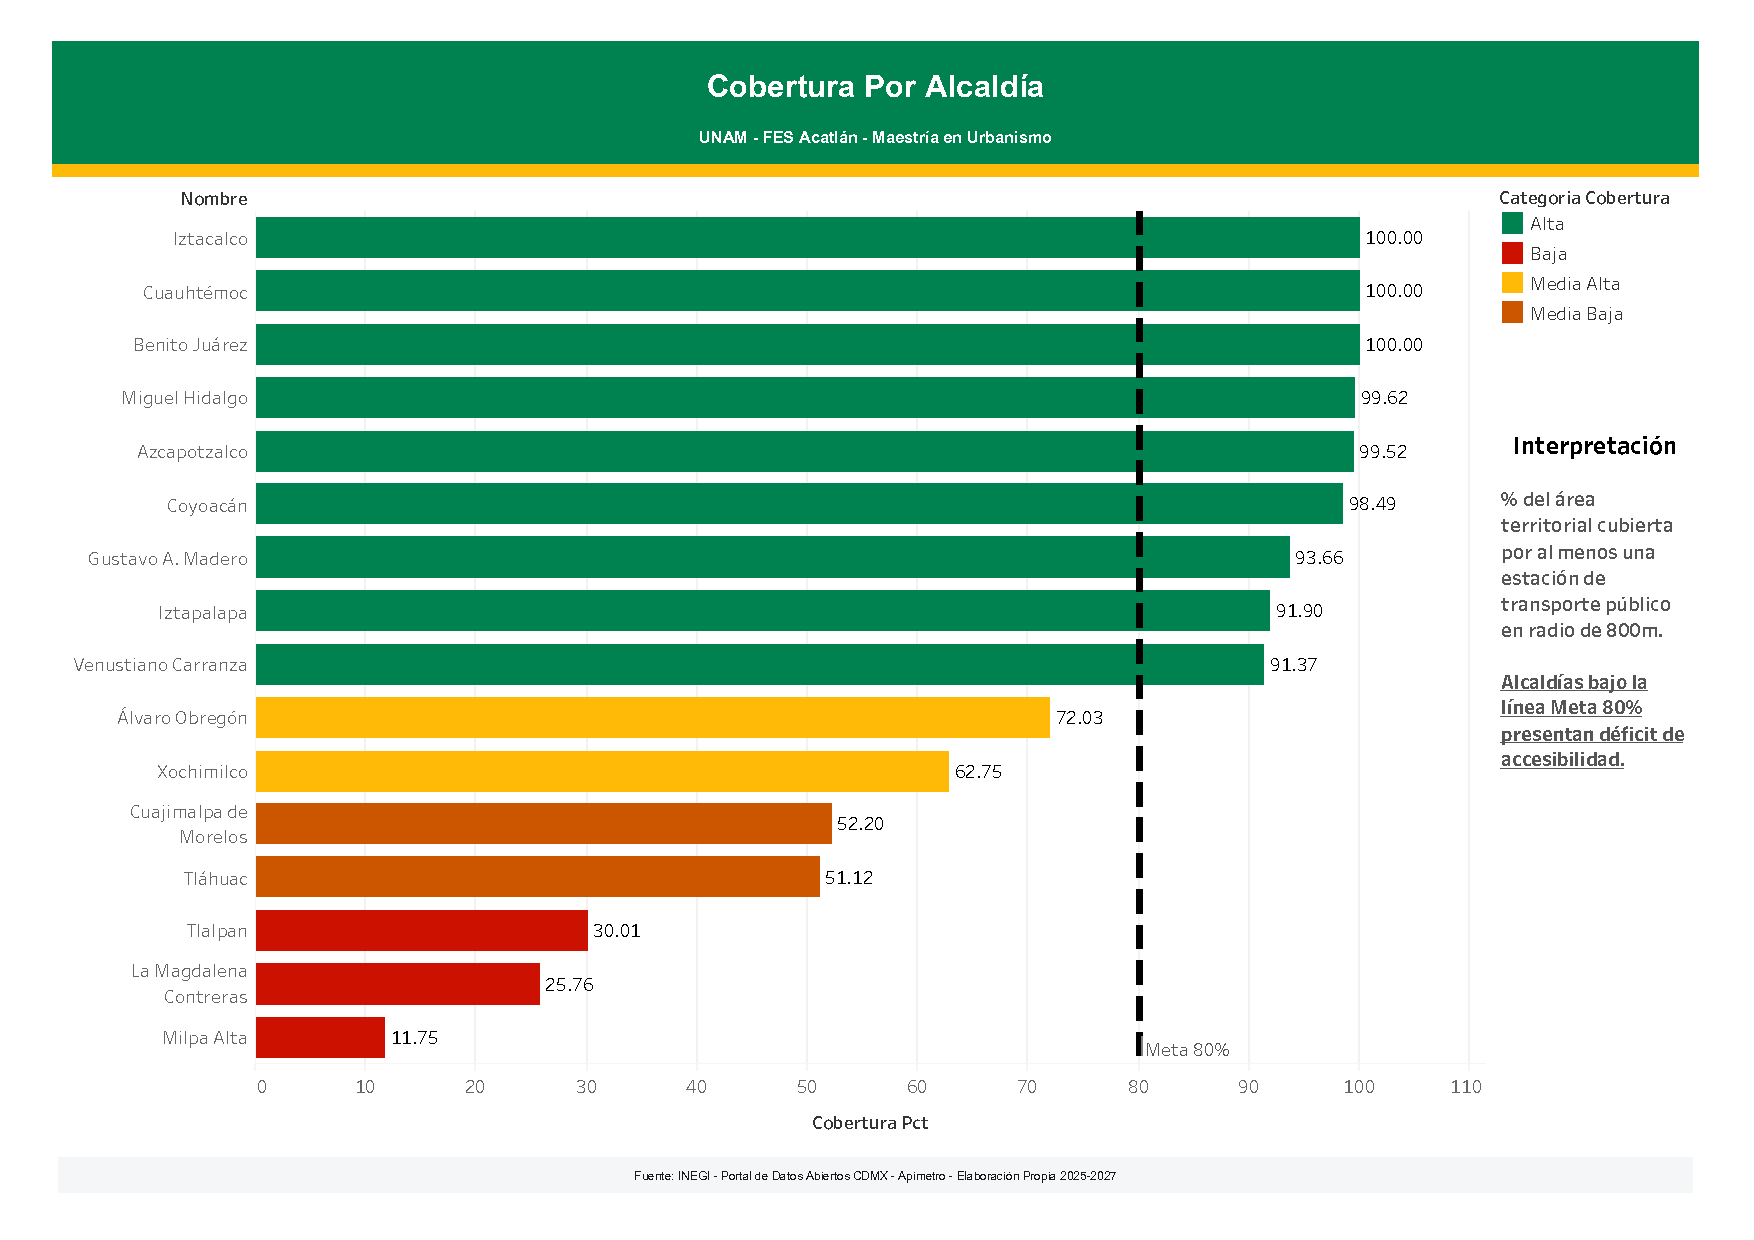
\includegraphics[width=0.9\textwidth]{Figures/Mapas/Tableau_Resources/RedActual/VFTModel/UniGrafica/Grafica_VFTModel_2026_Cobertura_alcaldia}
  \caption[Nivel de cobertura $C$ por alcaldía y municipio de la \zmvm{}]{Ranking
  de las 141~demarcaciones de la \zmvm{} ordenadas por nivel de cobertura espacial
  $C$. Identifica las alcaldías y municipios con mayor déficit de acceso estructurado
  al transporte público.}
  \label{fig:anx-f-tab-vft-cobertura-alcaldia}
  \fuentefigura{Elaboración propia con \textbf{Tableau Desktop 2026.1};
    fuente de datos: \textbf{VFTModel} vía \textsc{api} GeoProxy.}
\end{figure}

% --- F.3.6 -------------------------------------------------------------------
\subsection{Gráfica: Fuerza Capilar — Ranking de Nodos}
\label{anx:f-tab-vft-fc-ranking}

\begin{figure}[htb]
  \centering
  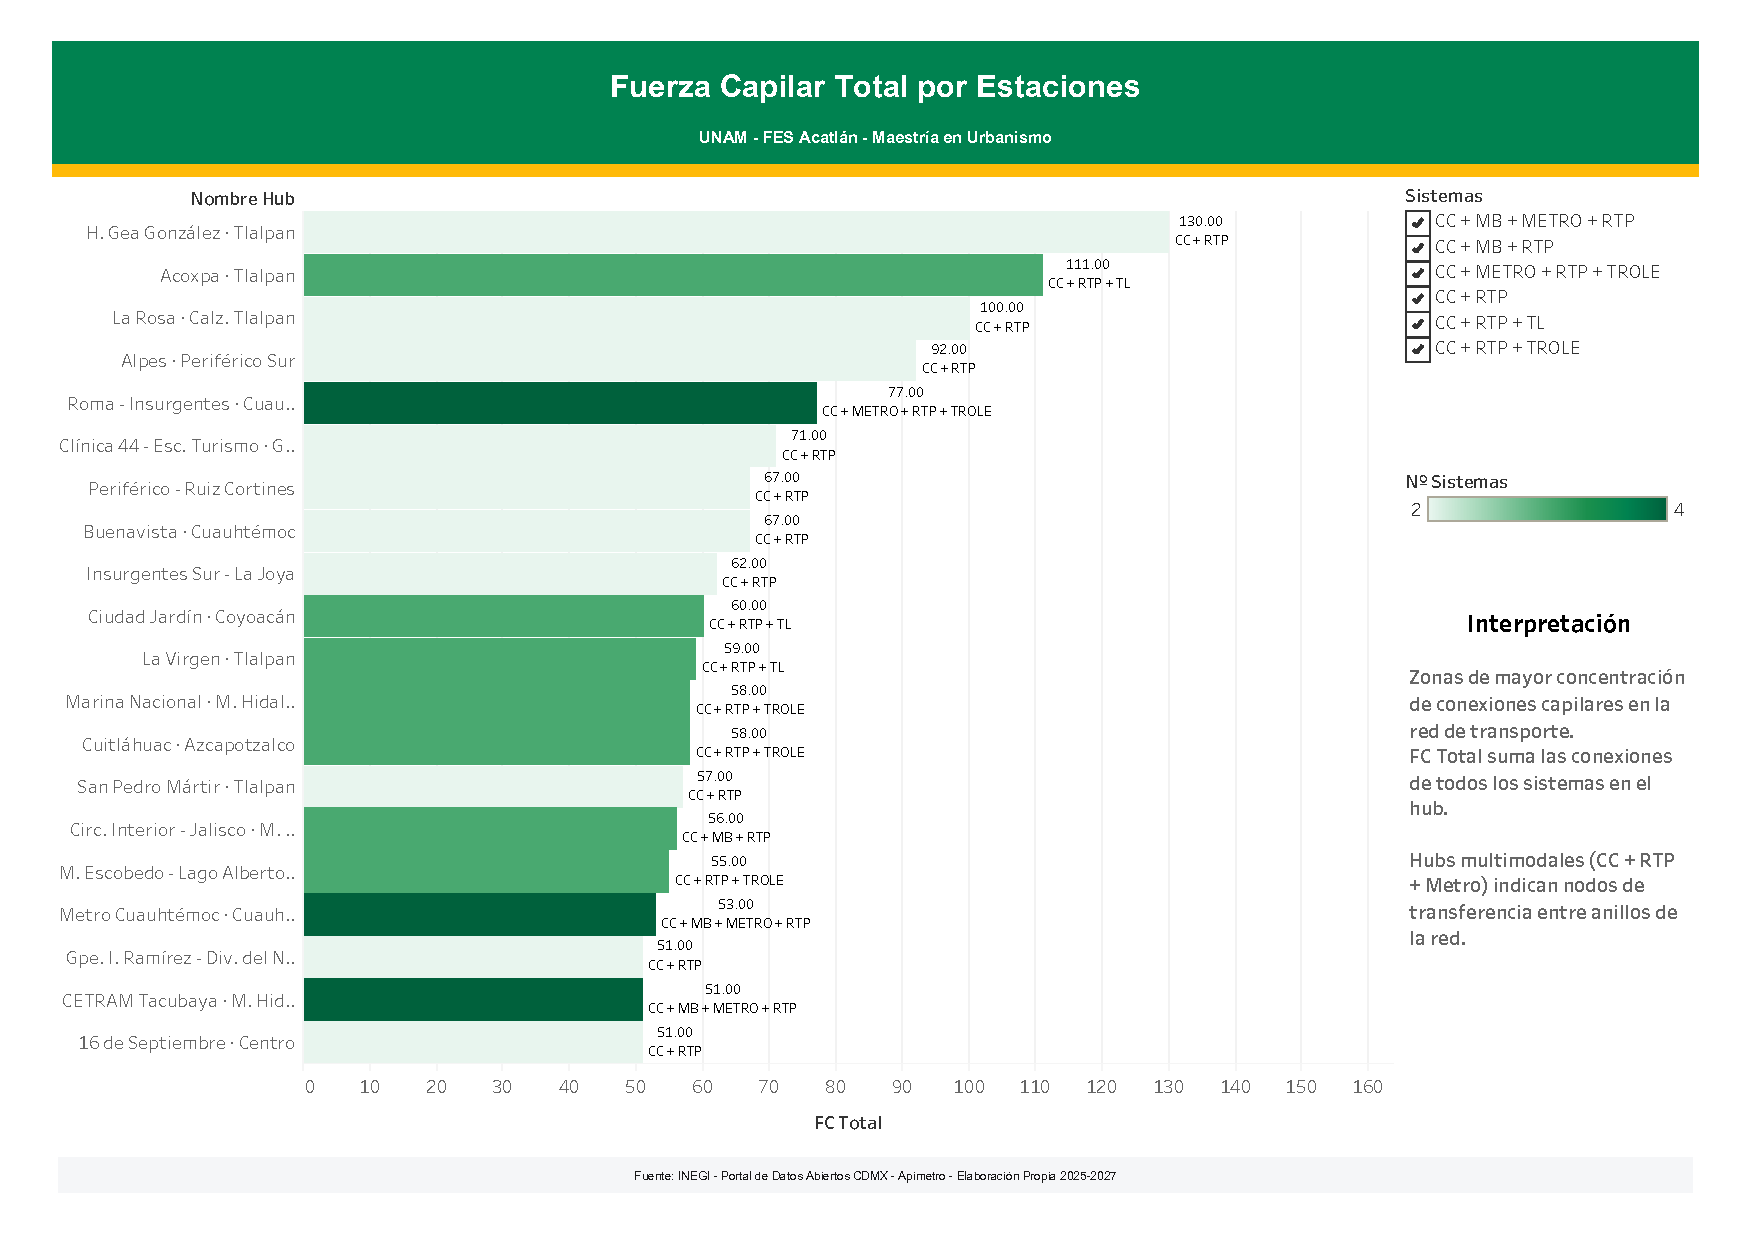
\includegraphics[width=0.9\textwidth]{Figures/Mapas/Tableau_Resources/RedActual/VFTModel/UniGrafica/Grafica_VFTModel_2026_Fuerza_capilar}
  \caption[Ranking de nodos por Fuerza Capilar $FC_h$]{Los veinte macrohubs con
  mayor valor de Fuerza Capilar $FC_h$ en la red de la \zmvm{}, con indicación del
  sistema de transporte predominante en cada hub. Muestra la concentración de la
  conectividad modal en puntos geográficos específicos de la red.}
  \label{fig:anx-f-tab-vft-fc-ranking}
  \fuentefigura{Elaboración propia con \textbf{Tableau Desktop 2026.1};
    fuente de datos: \textbf{VFTModel} vía \textsc{api} GeoProxy.}
\end{figure}

% --- F.3.7 -------------------------------------------------------------------
\subsection{Gráfica: Factor de Desviación — Distribución}
\label{anx:f-tab-vft-df-dist}

\begin{figure}[htb]
  \centering
  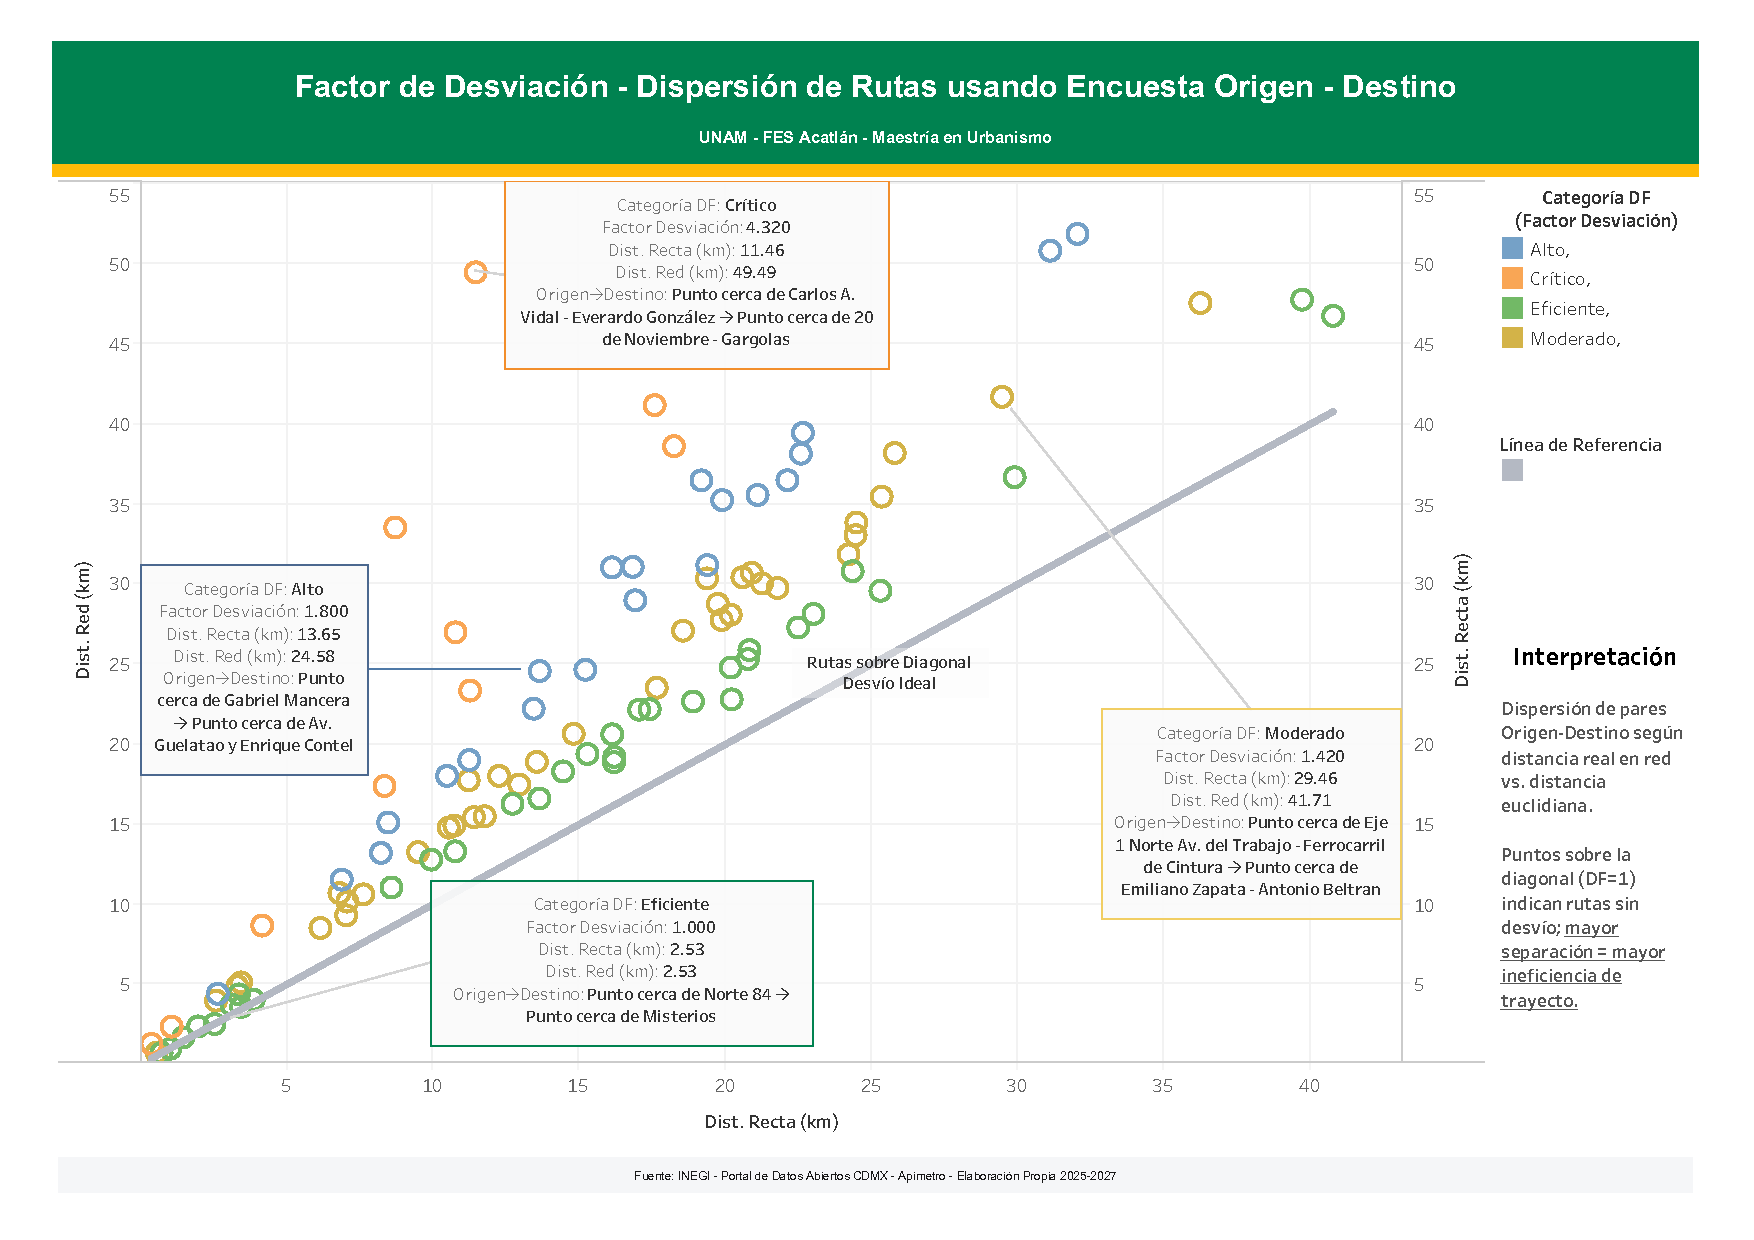
\includegraphics[width=0.9\textwidth]{Figures/Mapas/Tableau_Resources/RedActual/VFTModel/UniGrafica/Grafica_VFTModel_2026_Factor_desviacion}
  \caption[Distribución del Factor de Desviación $DI$ por alcaldía]{Distribución
  del indicador $DI$ entre las demarcaciones de la \zmvm{}, ordenadas por valor
  promedio. Un $DI$ cercano a~1.0 indica rutas casi directas; valores superiores
  a~2.0 señalan zonas donde el trazado de la red obliga a recorridos más del doble
  de la distancia euclidiana.}
  \label{fig:anx-f-tab-vft-df-dist}
  \fuentefigura{Elaboración propia con \textbf{Tableau Desktop 2026.1};
    fuente de datos: \textbf{VFTModel} vía \textsc{api} GeoProxy.}
\end{figure}

% --- F.3.8 -------------------------------------------------------------------
\subsection{Gráfica: Centralidad \texorpdfstring{$B(v)$}{B(v)} — Top Nodos}
\label{anx:f-tab-vft-bv-nodos}

\begin{figure}[htb]
  \centering
  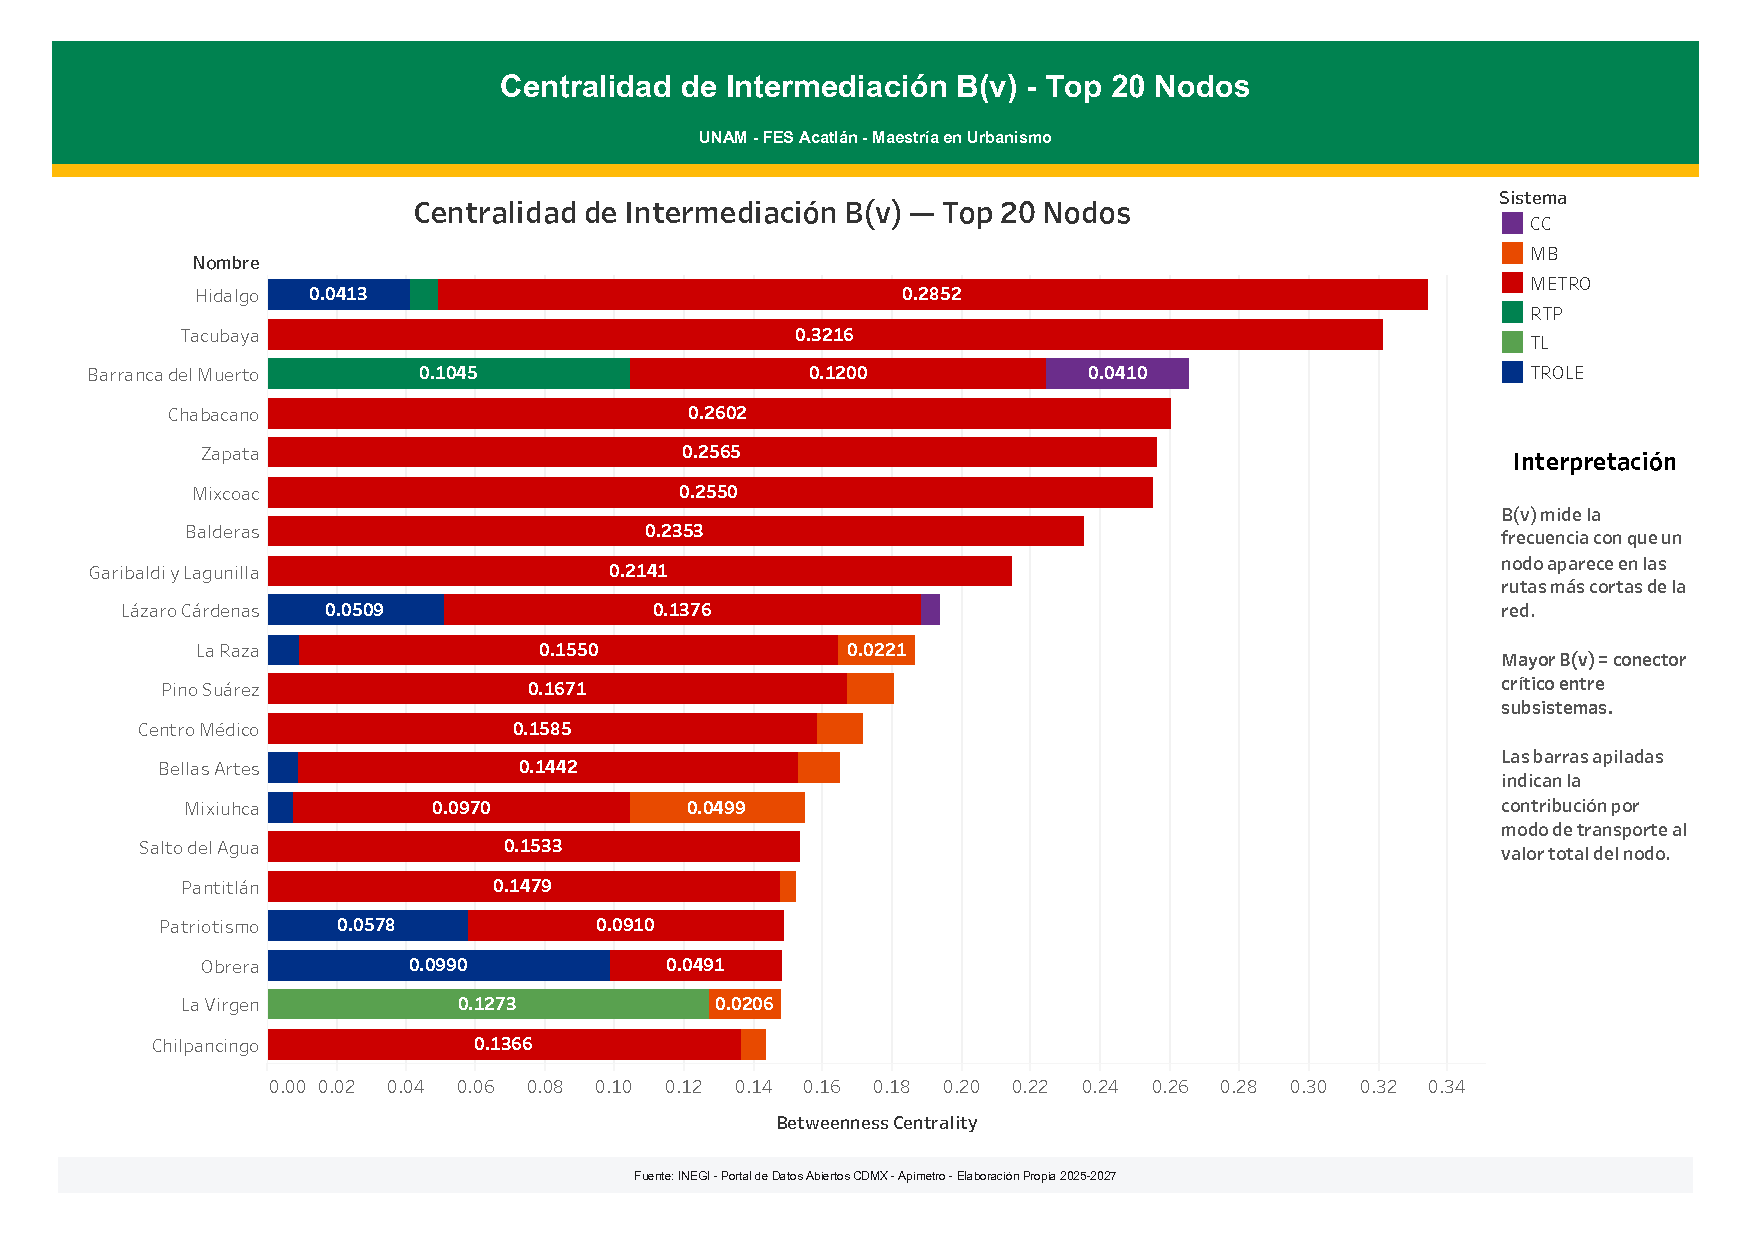
\includegraphics[width=0.9\textwidth]{Figures/Mapas/Tableau_Resources/RedActual/VFTModel/UniGrafica/Grafica_VFTModel_2026_Centralidad_Intermediacion_Nodos}
  \caption[Top~20 nodos por centralidad de intermediación $B(v)$]{Los veinte nodos
  de la red con mayor valor de centralidad de intermediación normalizada $B(v)$,
  calculado sobre la componente gigante de 10{,}561 nodos (corrida 2026-09-02).
  El valor de $B(v)$ indica la proporción de caminos mínimos de toda la red
  que atraviesan ese nodo.}
  \label{fig:anx-f-tab-vft-bv-nodos}
  \fuentefigura{Elaboración propia con \textbf{Tableau Desktop 2026.1};
    fuente de datos: \textbf{VFTModel} vía \textsc{api} GeoProxy.}
\end{figure}

% --- F.3.9 -------------------------------------------------------------------
\subsection{Gráfica: Centralidad \texorpdfstring{$B(v)$}{B(v)} — Por Sistema}
\label{anx:f-tab-vft-bv-sistema}

\begin{figure}[htb]
  \centering
  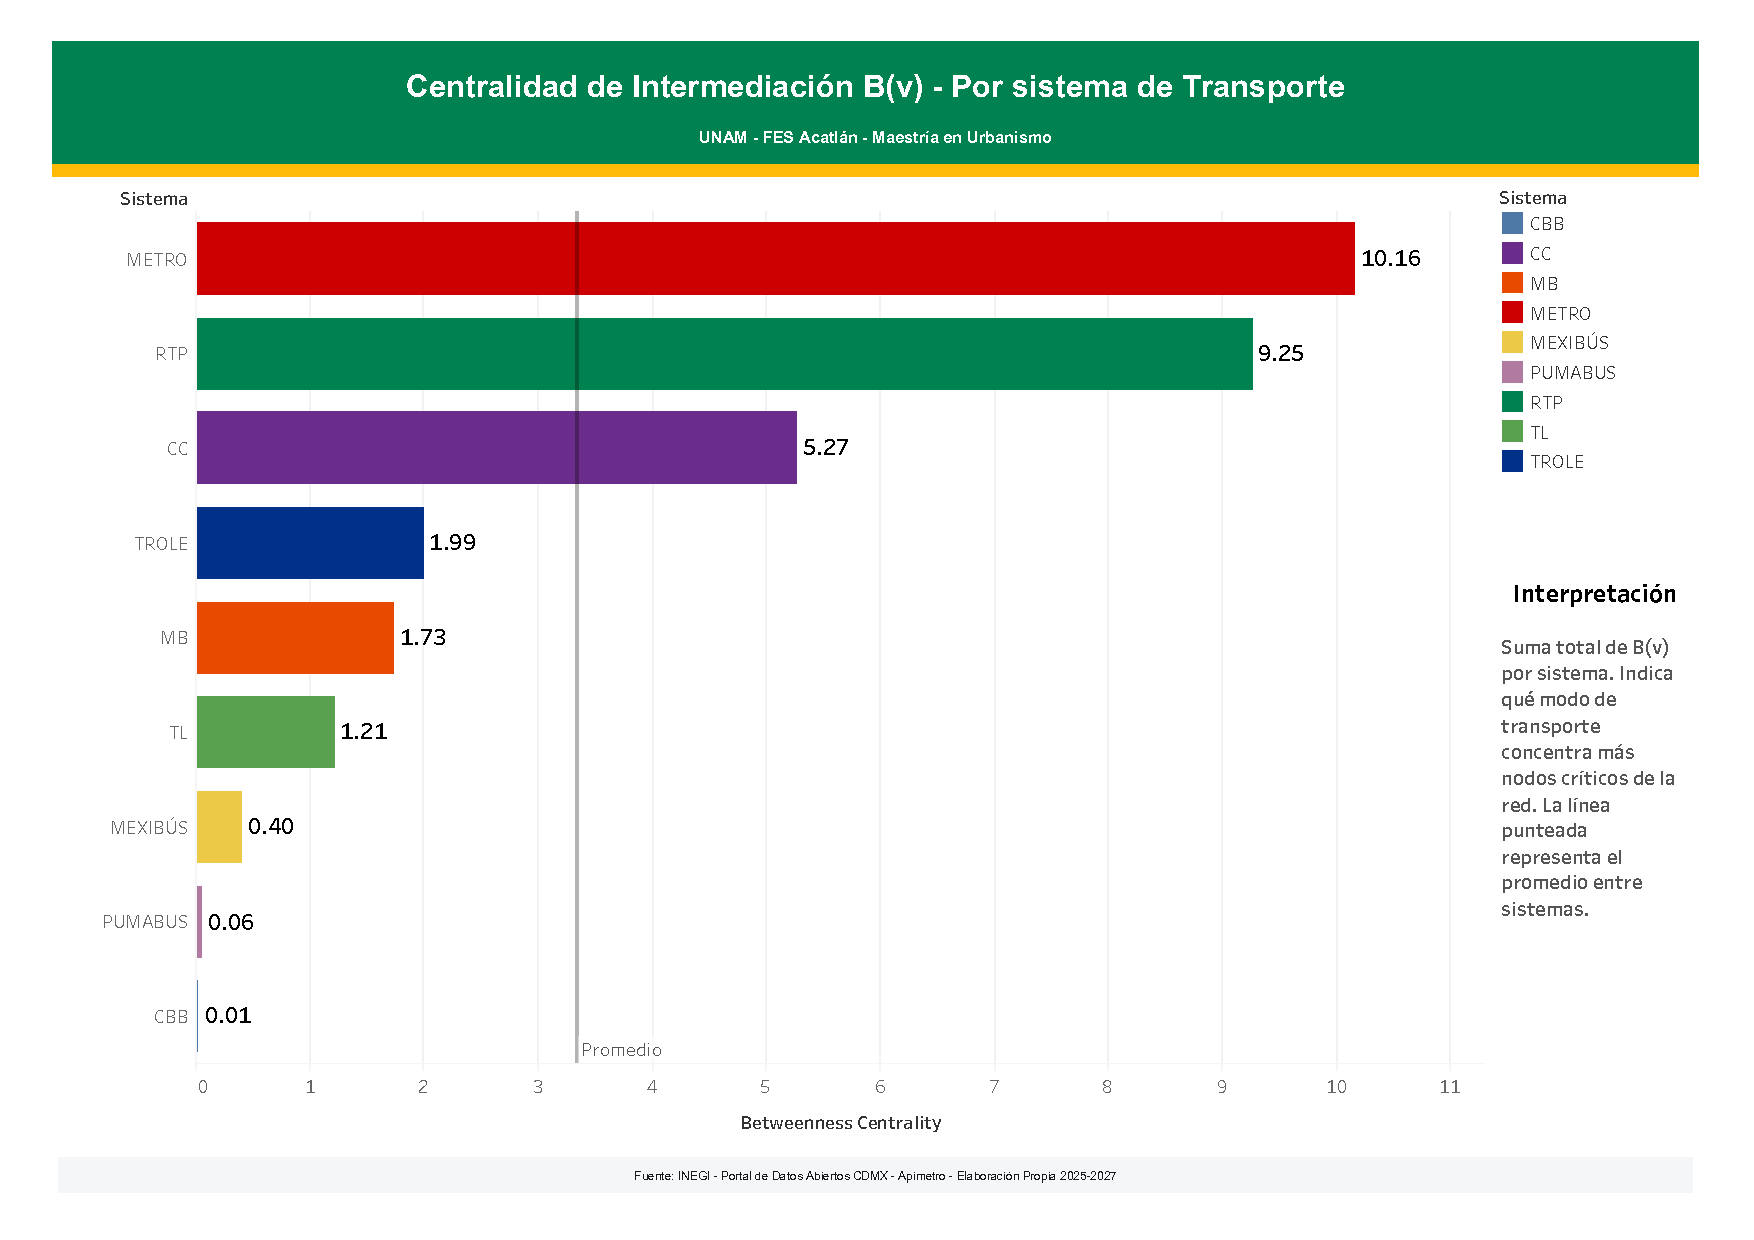
\includegraphics[width=0.9\textwidth]{Figures/Mapas/Tableau_Resources/RedActual/VFTModel/UniGrafica/Grafica_VFTModel_2026_Centralidad_Intermediacion_sistema}
  \caption[Centralidad de intermediación $B(v)$ acumulada por sistema de transporte]{Suma
  acumulada de centralidad de intermediación $B(v)$ agrupada por sistema de
  transporte. Revela qué sistemas concentran los nodos más críticos para la
  conectividad global de la red y cuáles tienen un papel estructural menor en la
  topología del grafo.}
  \label{fig:anx-f-tab-vft-bv-sistema}
  \fuentefigura{Elaboración propia con \textbf{Tableau Desktop 2026.1};
    fuente de datos: \textbf{VFTModel} vía \textsc{api} GeoProxy.}
\end{figure}
